% =====================================================================
%  Report: Parts I and II of the proposal
%  "Modularity Matrix Approach for Graph Learning?" (Anguluri and Dalal, Oct 2026)
%
%  Compiles with:   tectonic -X compile reports/2026-10-27_parts1_2_report.tex
%  Figures:         reports/figures/parts1_2/*.pdf, drawn from the cached learned
%                   graphs by modularity_graph_learning/report_figures.py
%  Numbers:         every number in the text and tables is printed by
%                   modularity_graph_learning/report_numbers.py (sections D to L;
%                   --part1 for Part I, --part2 for Part II)
%  This report supersedes, in presentation only, reports/2026-10-27_part1_lemma.tex,
%  which is kept unchanged as the working note.
% =====================================================================
\documentclass[11pt,a4paper]{article}

\usepackage[T1]{fontenc}
\usepackage[utf8]{inputenc}
\usepackage{lmodern}
\usepackage[margin=2.4cm]{geometry}
\usepackage{amsmath,amssymb,amsthm}
\usepackage{booktabs}
\usepackage{array}
\usepackage{enumitem}
\usepackage{xcolor}
\usepackage{microtype}
\usepackage{caption}
\usepackage{graphicx}
\usepackage{float}
\usepackage{tikz}
\usetikzlibrary{positioning,arrows.meta,calc}
\graphicspath{{figures/parts1_2/}}

\definecolor{BlueLink}{HTML}{1F4E79}
\definecolor{BadRed}{HTML}{B3261E}
\definecolor{GoodGreen}{HTML}{2F6F4E}
\definecolor{Panel2}{HTML}{F7F5F0}
\definecolor{PanelBlue}{HTML}{EEF3F8}
\definecolor{Rule}{HTML}{9AA3AD}

\usepackage[colorlinks=true,linkcolor=BlueLink,urlcolor=BlueLink,citecolor=BlueLink]{hyperref}
\emergencystretch=3em

\newcommand{\Lap}{\mathbf{L}}
\newcommand{\Wmat}{\mathbf{W}}
\newcommand{\Bmat}{\mathbf{B}}
\newcommand{\Dmat}{\mathbf{D}}
\newcommand{\Imat}{\mathbf{I}}
\newcommand{\Smat}{\mathbf{S}}
\newcommand{\Vmat}{\mathbf{V}}
\newcommand{\Umat}{\mathbf{U}}
\newcommand{\Jmat}{\mathbf{J}}
\newcommand{\dvec}{\mathbf{d}}
\newcommand{\uvec}{\mathbf{u}}
\newcommand{\vvec}{\mathbf{v}}
\newcommand{\xvec}{\mathbf{x}}
\newcommand{\bvec}{\mathbf{b}}
\newcommand{\wvec}{\mathbf{w}}
\newcommand{\zvec}{\mathbf{z}}
\newcommand{\one}{\mathbf{1}}
\newcommand{\tr}{\operatorname{tr}}
\newcommand{\Lsym}{\Lap_{\mathrm{sym}}}
\newcommand{\gdet}{\operatorname{gdet}}

\newtheorem{lemma}{Lemma}
\newtheorem{proposition}{Proposition}
\theoremstyle{remark}
\newtheorem*{remark}{Remark}

\captionsetup{font=small,labelfont=bf,width=.95\textwidth}
\setlist[itemize]{topsep=3pt,itemsep=2pt,parsep=0pt,leftmargin=1.3em}
\setlist[enumerate]{topsep=3pt,itemsep=2pt,parsep=0pt,leftmargin=1.8em}
\setlength{\parskip}{3pt}
\setcounter{tocdepth}{2}

% Shaded boxes: "aside" (grey, commentary) and "defn" (blue, a term being defined)
\newsavebox{\asidebox}
\newenvironment{aside}[1]
 {\par\vspace{2.5mm}\begin{lrbox}{\asidebox}%
  \begin{minipage}{\dimexpr\textwidth-16pt\relax}\small\textbf{#1}\par\vspace{1mm}}
 {\end{minipage}\end{lrbox}%
  \noindent\setlength{\fboxsep}{7pt}\setlength{\fboxrule}{.4pt}%
  \fcolorbox{Rule}{Panel2}{\usebox{\asidebox}}\par\vspace{2.5mm}}
\newsavebox{\defnbox}
\newenvironment{defn}[1]
 {\par\vspace{2mm}\begin{lrbox}{\defnbox}%
  \begin{minipage}{\dimexpr\textwidth-16pt\relax}\small\textcolor{BlueLink}{\textbf{#1}}\par\vspace{0.6mm}}
 {\end{minipage}\end{lrbox}%
  \noindent\setlength{\fboxsep}{6pt}\setlength{\fboxrule}{.4pt}%
  \fcolorbox{BlueLink!40}{PanelBlue}{\usebox{\defnbox}}\par\vspace{2mm}}

\begin{document}

% =====================================================================
%  Title page
% =====================================================================
\pagenumbering{Alph}
\begin{titlepage}
\centering
\vspace*{2.2cm}
{\Large Modularity Matrix Approach for Graph Learning?\par}
\vspace{6mm}
{\huge\bfseries Parts I and II:\\[2mm] what modularity adds to Laplacian\\[1mm] graph learning on stock returns\par}
\vspace{10mm}
{\large Jash Dalal\par}
\vspace{2mm}
{\normalsize Report on the proposal by Prof.\ Anguluri\quad$\cdot$\quad 27 October 2026\par}
\vspace{14mm}
\begin{minipage}{0.86\textwidth}
\small
\textbf{Abstract.} The proposal asks whether Newman's modularity matrix, the standard
tool for finding communities in a network, can improve the way Cardoso and Palomar
(2020) learn a network of stocks from their returns. This report answers its first two
parts. \emph{Part I}: under the paper's rule that every stock has total link weight 1,
the modularity matrix is an exact mirror image of the graph Laplacian, so modularity
adds nothing new; I prove the three claims of the proposal, show where the needed
condition fails, and confirm the mirror image on the paper's own learned graph, where it
holds to within the solver's tolerance. \emph{Part II}: the Laplacian learner already
removes the market's common movement on its own, exactly when all stocks have the same
beta. On the paper's S\&P data this built-in removal is enough, and four standard ways
of removing the market explicitly all make the result worse. In simulated markets where
betas vary within sectors, the built-in removal fails suddenly once beta inequality
passes a threshold, and explicit removal then fixes it. A two-step perturbation bound is
proved; its first step is realistic, its second is too loose to be useful here, and the
measured switch point is reported instead.
\end{minipage}
\vfill
{\small Code: \texttt{modularity\_graph\_learning/}. Every number is printed by
\texttt{report\_numbers.py}; every figure is drawn from the learned graphs by
\texttt{report\_figures.py}.\par}
\end{titlepage}

\pagenumbering{roman}
\tableofcontents
\clearpage
\pagenumbering{arabic}

% =====================================================================
\section{Introduction}\label{sec:intro}
% =====================================================================

\subsection{The starting point: learning a network of stocks}

Cardoso and Palomar (2020), \emph{Learning undirected graphs in financial markets}
(arXiv:2005.09958; ``Paper 1'' below), turn a table of daily stock returns into a
network. Each stock is a node; a link between two stocks carries a weight that says how
directly their returns are tied together once all the other stocks are accounted for.
The learned network is then read for structure: which groups of stocks hang together
(clusters), and how tightly the market as a whole is connected (used as a stress
indicator). Figure~\ref{fig:pipeline} shows the pipeline used throughout this report.

\begin{figure}[htbp]
\centering
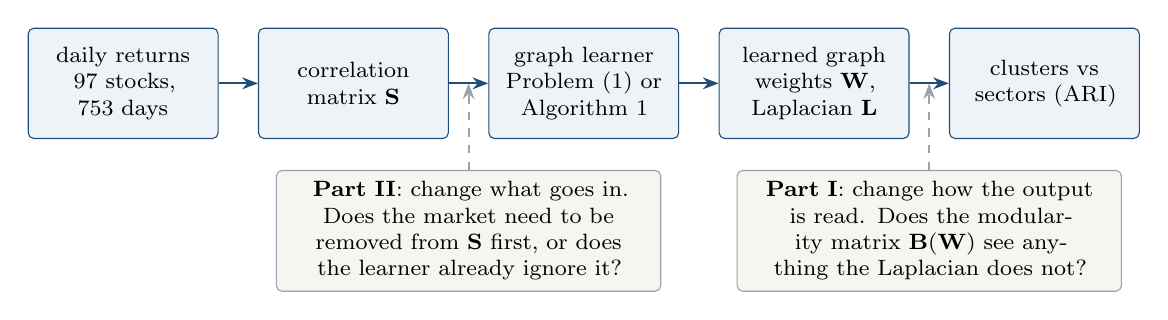
\begin{tikzpicture}[
  box/.style={draw=BlueLink,fill=PanelBlue,rounded corners=2pt,align=center,
              font=\footnotesize,minimum height=14mm,text width=22mm,inner sep=3pt},
  part/.style={draw=Rule,fill=Panel2,rounded corners=2pt,align=center,
              font=\footnotesize,text width=46mm,inner sep=4pt},
  arr/.style={-{Stealth[length=2mm]},thick,BlueLink}]
\node[box] (r) {daily returns\\97 stocks, 753 days};
\node[box,right=5mm of r] (s) {correlation\\matrix $\Smat$};
\node[box,right=5mm of s] (g) {graph learner\\Problem (1) or\\Algorithm 1};
\node[box,right=5mm of g] (l) {learned graph\\weights $\Wmat$,\\Laplacian $\Lap$};
\node[box,right=5mm of l] (c) {clusters vs\\sectors (ARI)};
\draw[arr] (r) -- (s); \draw[arr] (s) -- (g); \draw[arr] (g) -- (l); \draw[arr] (l) -- (c);
\node[part,below=11mm of $(s)!0.5!(g)$] (p2) {\textbf{Part II}: change what goes in.
  Does the market need to be removed from $\Smat$ first, or does the learner already
  ignore it?};
\node[part,below=11mm of $(l)!0.5!(c)$] (p1) {\textbf{Part I}: change how the output
  is read. Does the modularity matrix $\Bmat(\Wmat)$ see anything the Laplacian does
  not?};
\draw[arr,Rule,dashed] (p2.north) -- ($(s)!0.5!(g)$ |- s.south);
\draw[arr,Rule,dashed] (p1.north) -- ($(l)!0.5!(c)$ |- l.south);
\end{tikzpicture}
\caption{The pipeline of Paper 1 as used in this report, and where the two parts of the
proposal act on it.}
\label{fig:pipeline}
\end{figure}

\subsection{What the proposal asks}

The proposal, \emph{Modularity Matrix Approach for Graph Learning?}, starts from an
observation: the graph Laplacian that Paper 1 learns, and the modularity matrix that
network science uses to find communities, are built from the same weights. It asks, in
three parts, whether modularity can add something.
\begin{itemize}
\item \textbf{Part I} asks what modularity says about the graphs Paper 1 already
  learns. Paper 1's clustering method forces every stock to have total link weight 1;
  under that rule the proposal conjectures that the two matrices are mirror images and
  lists three consequences, labelled (a), (b) and (c).
\item \textbf{Part II} asks about the market. Modularity methods subtract an explicit
  model of ``what everything has in common'' (a \emph{null model}) before looking for
  groups. Paper 1 never does. The proposal conjectures that the Laplacian removes the
  market on its own, and asks when that is enough, given that stocks react to the
  market by different amounts (their \emph{betas}).
\item \textbf{Part III} proposes a new learner with a modularity term in place of the
  unit-degree rule. It is not covered here: as written its objective is unbounded below
  (reported in the 18 October note), and it waits on a choice of repair.
\end{itemize}

\subsection{Findings at a glance}

\begin{aside}{Part I: under the unit-degree rule, modularity adds nothing new}
\begin{itemize}
\item The modularity matrix is the Laplacian reflected: $\Bmat=\Imat-\Lap-\one\one^\top/p$,
  so every eigenvalue $\lambda$ of $\Lap$ becomes $1-\lambda$ of $\Bmat$ with the same
  eigenvector. All three claims follow; they are proved in Section~\ref{sec:lemma}.
\item Claim (b) needs a condition ($\lambda_k\le1$). I give its exact form without the
  condition and two small graphs where it fails (Section~\ref{sec:role}).
\item On Paper 1's own learned graph every eigenvalue pair matches the mirror image to
  within $0.006$, and the modularity matrix finds exactly the three sectors
  (Section~\ref{sec:fig2}).
\item Without the unit-degree rule the algebra stops holding, but the clusters do not
  change; a degree-normalised version of the identity holds for any degrees
  (Sections~\ref{sec:classify} and~\ref{sec:sweep}).
\end{itemize}
\end{aside}
\begin{aside}{Part II: the market is removed for free, unless betas cut across groups}
\begin{itemize}
\item The learner only ever sees returns with each day's average removed. Equal betas
  are therefore removed exactly; unequal betas leave a penalty on links between
  high-beta and low-beta stocks (Section~\ref{sec:implicit}).
\item On the S\&P data, Algorithm 1 recovers the sectors exactly, and every explicit
  market removal does worse (ARI 0.830 to 0.896 against 1.000), because here betas
  follow sectors (Section~\ref{sec:real}).
\item In simulated markets with high and low betas inside every sector, the clusters
  switch from sectors to beta groups over a narrow range of beta inequality; explicit
  removal recovers the sectors every time (Section~\ref{sec:synthetic}).
\item A two-step perturbation bound is proved. Step 1 is within a factor 1.65 to 4.84
  of the truth; Step 2 (Davis-Kahan) is too loose to be informative. The switch happens
  when the change in the graph reaches the size of its eigengap (Section~\ref{sec:boundcheck}).
\end{itemize}
\end{aside}

\subsection{How to read this report}

Section~\ref{sec:background} introduces every object and term used later, each with a
small worked picture; readers who know spectral graph theory can skip to
Section~\ref{sec:part1}. Terms are also collected in the glossary
(Appendix~\ref{app:glossary}). Each result carries one of three labels:
\emph{reproduced} (the claim holds in our computations), \emph{partial} (it holds with
qualifications that are stated), or \emph{not reproduced / not supported}. Negative
results are reported as prominently as positive ones, and every deviation from the
paper or the proposal is listed in Section~\ref{sec:status}. The suggested next steps
are suggestions; which to pursue is the professor's decision.

% =====================================================================
\section{Background: the objects and the terms}\label{sec:background}
% =====================================================================

\subsection{The data}\label{sec:data}

Paper 1's clustering experiment uses $p=97$ stocks from the S\&P 500 in three sectors:
52 Industrials, 28 Consumer Staples and 17 Energy. For each stock $i$ and trading day
$t$ the \emph{log return} $x_{t,i}=\log(P_{t,i}/P_{t-1,i})$ is the day's relative price
change. We use the paper's window of $T=753$ trading days, 5 January 2016 to 31 December
2018.

\begin{defn}{Correlation matrix $\Smat$}
The $p\times p$ matrix whose entry $S_{ij}$ is the sample correlation between the daily
returns of stocks $i$ and $j$ over the $T$ days. $S_{ii}=1$; values near 1 mean the two
stocks rise and fall together. $\Smat$ is the only input the learners see.
\end{defn}

\begin{figure}[htbp]
\centering
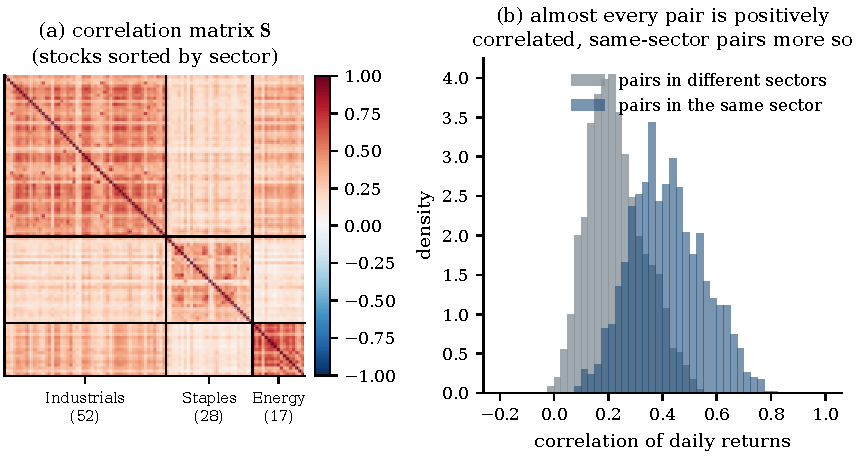
\includegraphics[width=\textwidth]{fig05_data.pdf}
\caption{The input. (a) The correlation matrix with stocks sorted by sector: the three
darker diagonal blocks are the sectors, but nearly every entry is positive, because all
stocks share the market's daily ups and downs. (b) Same-sector pairs are more correlated
than cross-sector pairs, but the two distributions overlap heavily.}
\label{fig:data}
\end{figure}

Figure~\ref{fig:data} shows the two features that drive this report. The sectors are
visible, which is what a good learner should recover. And everything is positively
correlated, which is the market factor that Part II is about.

\subsection{Graphs, weights and degrees}

\begin{defn}{Weighted graph}
A set of $p$ nodes (here, stocks) and a symmetric weight matrix $\Wmat$ with
$W_{ij}=W_{ji}\ge0$ and $W_{ii}=0$. $W_{ij}>0$ means there is a link (an \emph{edge})
between $i$ and $j$, and its size is the link's strength.
\end{defn}
\begin{defn}{Degree $d_i$}
The total weight of node $i$'s links, $d_i=\sum_jW_{ij}$. Collected in the vector
$\dvec=\Wmat\one$, where $\one$ is the vector of all ones, and in the diagonal matrix
$\Dmat=\operatorname{Diag}(\dvec)$. The total weight of the graph is
$2m=\sum_id_i=\one^\top\dvec$ (each edge counted from both ends).
\end{defn}
A graph is \emph{regular} if every degree is the same number $c$, and has
\emph{unit degree} if $c=1$. A \emph{connected component} is a group of nodes joined to
each other by paths of edges but with no edge to any node outside the group.

\subsection{The graph Laplacian}\label{sec:laplacian}

\begin{defn}{Graph Laplacian $\Lap$}
$\Lap=\Dmat-\Wmat$: the degrees on the diagonal and minus the weights off it. For any
vector $\xvec$ with one value per node,
\begin{equation}\label{eq:quad}
  \xvec^\top\Lap\xvec=\sum_{i<j}W_{ij}(x_i-x_j)^2 .
\end{equation}
\end{defn}

Equation~\eqref{eq:quad} is the key to everything below. It says that $\Lap$ measures how
much a node signal $\xvec$ \emph{changes across edges}: each edge charges its weight
times the squared difference of its two ends. A signal that is constant on tightly
linked groups and changes only across weak links is cheap; a signal that alternates
between neighbours is expensive (Figure~\ref{fig:laplacian}). In particular
$\Lap\one=\mathbf0$: moving every node by the same amount costs nothing.

\begin{figure}[htbp]
\centering
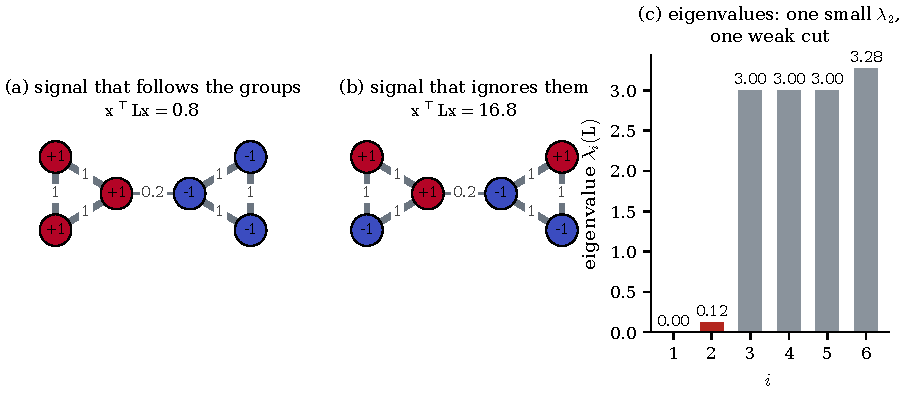
\includegraphics[width=\textwidth]{fig02_laplacian.pdf}
\caption{The Laplacian on a toy graph: two triangles (edge weights 1) joined by a weak
edge (weight 0.2). (a) A signal that is $+1$ on one triangle and $-1$ on the other only
changes across the weak edge, so $\xvec^\top\Lap\xvec$ is small. (b) A signal that
alternates between neighbours is expensive. (c) The eigenvalues of $\Lap$: 0 (the
constant signal), then one small eigenvalue $\lambda_2=0.12$ whose eigenvector is the
signal in (a), then a jump.}
\label{fig:laplacian}
\end{figure}

\subsection{What the eigenvalues of a Laplacian say}\label{sec:eigen}

$\Lap$ is symmetric and, by \eqref{eq:quad}, positive semidefinite, so it has real
eigenvalues $0=\lambda_1\le\lambda_2\le\dots\le\lambda_p$ with orthonormal eigenvectors.
Each eigenvector is a node signal, and its eigenvalue is its cost
\eqref{eq:quad}. Three facts are used repeatedly.
\begin{itemize}
\item \textbf{Zero eigenvalues count components.} A signal that is constant on each
  component costs nothing, so a graph with $k$ components has exactly $k$ zero
  eigenvalues, that is, $\operatorname{rank}(\Lap)=p-k$ (Figure~\ref{fig:components}a).
\item \textbf{Small eigenvalues mark weak cuts.} If the components are joined by weak
  links, the zeros become small positive eigenvalues, still well separated from the
  rest (Figure~\ref{fig:components}b). $\lambda_2$ is called the \emph{algebraic
  connectivity}: it is 0 exactly when the graph is disconnected, and small when the
  graph is close to splitting. Its eigenvector is the \emph{Fiedler vector}.
\item \textbf{The eigengap measures how clear the groups are.} The gap
  $\lambda_{k+1}-\lambda_k$ between the $k$ small eigenvalues and the rest says how
  sharply the graph separates into $k$ groups. It reappears in Part II, where it decides
  how much perturbation the groups can survive.
\end{itemize}

\begin{figure}[htbp]
\centering
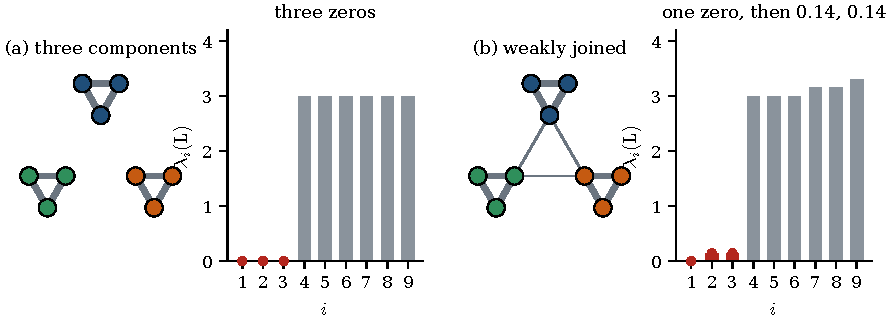
\includegraphics[width=\textwidth]{fig03_components.pdf}
\caption{(a) Three separate triangles: three zero eigenvalues (red), one per component.
(b) The same triangles joined by weak edges (weight 0.15): one zero, then two small
eigenvalues, then a gap. Counting small eigenvalues counts groups.}
\label{fig:components}
\end{figure}

\begin{defn}{Spectral clustering, $k$-means and ARI}
\emph{Spectral clustering} gives each node the coordinates it has in the $k$ eigenvectors
with the smallest eigenvalues, then groups the nodes with \emph{$k$-means}, which splits
points into $k$ groups so that each point is close to its group's average. For a graph
with $k$ components this simply returns the components.
The \emph{adjusted Rand index} (ARI) compares two ways of grouping the same items: 1 means
identical groupings, about 0 means no more agreement than chance, and negative values
mean less. Throughout, ARI compares learned clusters with the sector labels.
\end{defn}

\subsection{Modularity and the modularity matrix}\label{sec:modularity}

Network science finds communities differently. Newman's \emph{modularity} asks whether a
group has more internal weight than one would expect by chance, and so needs a model of
``chance'': a \emph{null model}.

\begin{defn}{Null model and modularity matrix $\Bmat$}
The standard (configuration) null model keeps every node's degree and wires the weight
at random, so the expected weight between $i$ and $j$ is $d_id_j/2m$. The
\emph{modularity matrix} is observed minus expected,
\[
  \Bmat=\Wmat-\frac{\dvec\dvec^\top}{2m},\qquad B_{ij}=W_{ij}-\frac{d_id_j}{2m}.
\]
For a split of the nodes into groups, the \emph{modularity} $Q$ adds up $B_{ij}$ over
pairs in the same group (divided by $2m$): positive $Q$ means the groups hold more weight
than chance.
\end{defn}

Maximising $Q$ exactly is hard, so it is relaxed: replacing group labels by real-valued
vectors, the best two-way split is read from the top eigenvector of $\Bmat$, and the best
$k$-way split from the top $k-1$ eigenvectors, through the \emph{relaxed modularity}
$\max\tr(\Umat^\top\Bmat\Umat)$ over $p\times(k-1)$ matrices $\Umat$ with orthonormal
columns. Write the eigenvalues of $\Bmat$ in decreasing order,
$\mu_1\ge\mu_2\ge\dots\ge\mu_p$. Since $\Bmat\one=\mathbf0$, 0 is always one of them.
Newman's \emph{divisibility test} says a network is worth splitting at all only if
$\mu_1>0$ (Figure~\ref{fig:modularity}).

\begin{figure}[htbp]
\centering
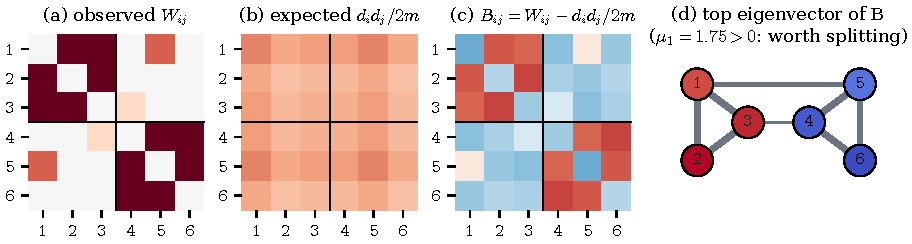
\includegraphics[width=\textwidth]{fig04_modularity.pdf}
\caption{Modularity on the toy graph of Figure~\ref{fig:laplacian} with one extra
cross edge (nodes 1 and 5). (a) Observed weights. (b) Weights expected by chance given
the degrees. (c) Their difference $\Bmat$: positive (red) inside the triangles, negative
(blue) between them. (d) The top eigenvector of $\Bmat$ separates the two triangles, and
$\mu_1>0$ says splitting is worthwhile.}
\label{fig:modularity}
\end{figure}

The parallel with Section~\ref{sec:eigen} is the starting point of the proposal: the
Laplacian finds groups through its \emph{smallest} eigenvalues, modularity through its
\emph{largest}. Part I asks when these are the same thing.

\begin{defn}{Normalised versions}
Dividing by the degrees gives the \emph{normalised Laplacian}
$\Lsym=\Imat-\Dmat^{-1/2}\Wmat\Dmat^{-1/2}$ and the \emph{normalised modularity matrix}
$\Bmat_n=\Dmat^{-1/2}\Bmat\Dmat^{-1/2}$. They treat a weakly connected node and a strongly
connected node on the same footing, and appear in Section~\ref{sec:classify}.
\end{defn}

\subsection{The learners of Paper 1}\label{sec:learners}

Paper 1 models the returns as a \emph{Gaussian Markov random field}: Gaussian with
precision (inverse covariance) matrix $\Lap$. In such a model $L_{ij}=-W_{ij}$ is nonzero
exactly when stocks $i$ and $j$ are linked after accounting for all the others. Fitting
the model to $\Smat$ by maximum likelihood gives an objective with two parts, both in
terms of $\Lap$.

\begin{defn}{Problem (1): the basic learner}
\[
  \min_{\Lap\text{ a Laplacian}}\ \tr(\Lap\Smat)-\log\gdet(\Lap)+\beta\sum_{i<j}W_{ij}.
\]
$\tr(\Lap\Smat)=\sum_{i<j}W_{ij}(S_{ii}+S_{jj}-2S_{ij})$ is the \emph{data fit}: by
\eqref{eq:quad} it is small when strong links join stocks whose returns move together.
$\gdet$, the \emph{generalised determinant}, is the product of the nonzero eigenvalues;
the $-\log\gdet$ term stops all weights collapsing to zero. The last term, with
\emph{sparsity weight} $\beta$, favours fewer links. We use $\beta=10$, the setting of
the paper's Fig.~1. Problem (1) is convex and returns one connected graph; clusters are
then read by spectral clustering.
\end{defn}

\begin{defn}{Algorithm 1: the $k$-component learner}
Paper 1's Algorithm 1 adds two requirements: the graph must have exactly $k$ components
(here $k=3$, one per sector), and every degree must be 1, $\operatorname{diag}(\Lap)=\one$,
so that no stock can be cut off with zero links. The component requirement is imposed
through \emph{Ky Fan's theorem}: the sum of the $k$ smallest eigenvalues of $\Lap$
equals $\min\tr(\Vmat^\top\Lap\Vmat)$ over $p\times k$ matrices $\Vmat$ with orthonormal
columns, and adding $\eta\tr(\Vmat^\top\Lap\Vmat)$ to the objective pushes those $k$
eigenvalues to 0. The algorithm alternates between choosing $\Vmat$ (the bottom $k$
eigenvectors of the current $\Lap$) and re-solving for $\Lap$. Clusters are its
connected components.
\end{defn}

Three implementation choices are ours and recorded as deviations. The paper does not
report the Fan weight; we use $\eta=300$. The degree rule is imposed as a penalty
$\tfrac\rho2\lVert\operatorname{diag}(\Lap)-\one\rVert^2$ with $\rho=100$, so learned
degrees are close to 1 but not exactly 1. And Algorithm 1 starts from the Problem (1)
graph: from the paper's uniform starting graph the components are set by round-off
error and do not match the sectors (18 October note).

% =====================================================================
\section{Part I: modularity under the unit-degree rule}\label{sec:part1}
% =====================================================================

\subsection{The question}

Algorithm 1 forces every degree to be 1. With $\dvec=\one$ the null model's expected
weight $d_id_j/2m$ becomes the same number, $1/p$, for every pair: chance predicts a
uniform graph. So the modularity matrix no longer depends on the degrees at all, and it
is natural to suspect it carries no information beyond $\Lap$. The proposal makes this
precise in three claims. In words:
\begin{itemize}
\item[(a)] \textbf{Counting clusters.} The graph has $k$ components exactly when $\Bmat$
  has the eigenvalue 1 repeated $k-1$ times. So modularity counts clusters the same way
  the Laplacian does.
\item[(b)] \textbf{Algorithm 1 is secretly maximising modularity.} The Ky Fan term that
  Algorithm 1 minimises equals a constant minus the relaxed $(k-1)$-way modularity,
  provided $\lambda_k\le1$.
\item[(c)] \textbf{The stress indicator is a modularity test.} The top modularity
  eigenvalue is $\mu_1=\max\{0,1-\lambda_2\}$. Paper 1 tracks the algebraic connectivity
  $\lambda_2$ of rolling-window graphs as a market-stress indicator, and our replication
  of its trading rule invests only when $\lambda_2<\tau=1$. Claim (c) says that, under
  unit degree, this rule is exactly Newman's divisibility test $\mu_1>0$.
\end{itemize}

\subsection{The reflection lemma and the three claims}\label{sec:lemma}

When $\dvec=\one$: $\Dmat=\Imat$, the total weight is $2m=p$, and so
\begin{equation}\label{eq:B}
  \Bmat=\Wmat-\tfrac1p\one\one^\top=\Imat-\Lap-\tfrac1p\one\one^\top .
\end{equation}
This is a property of the \emph{learned} graph, not an assumption about the data. The
eigenvalues of a unit-degree Laplacian lie in $[0,2]$, since $\Wmat=\Imat-\Lap$ has rows
of absolute sum 1 and hence eigenvalues in $[-1,1]$.

\begin{lemma}[Reflection]\label{lem:core}
Under $\dvec=\one$, take an orthonormal eigenbasis of $\Lap$ with $\vvec_1=\one/\sqrt p$
and $\Lap\vvec_i=\lambda_i\vvec_i$. Then $\Bmat\vvec_1=\mathbf0$ and
$\Bmat\vvec_i=(1-\lambda_i)\vvec_i$ for $i\ge2$. So $\Lap$ and $\Bmat$ have the same
eigenvectors, and $\operatorname{spec}(\Bmat)=\{0\}\cup\{1-\lambda_i:\ i=2,\dots,p\}$.
\end{lemma}
\begin{proof}
Such a basis exists because $\Lap\one=\mathbf0$. By \eqref{eq:B},
$\Bmat\vvec_1=\vvec_1-\mathbf0-\vvec_1=\mathbf0$. For $i\ge2$, $\vvec_i\perp\one$, so
the last term of \eqref{eq:B} vanishes and $\Bmat\vvec_i=\vvec_i-\lambda_i\vvec_i$.
\end{proof}

In words: apart from the direction $\one$ (``all stocks move together''), which both
matrices ignore, $\Bmat$ is $\Lap$ reflected through $\tfrac12$. Cheap cuts of the
Laplacian become valuable splits for modularity.

\begin{proposition}\label{prop:lemma}
Under $\dvec=\one$:
\begin{enumerate}[label=(\alph*)]
\item $\operatorname{rank}(\Lap)=p-k$ if and only if $\Bmat$ has eigenvalue 1 with
  multiplicity exactly $k-1$. Moreover $\mu_1\le1$.
\item For every $k\ge2$,
  \[
    \underbrace{\min_{\Vmat^\top\Vmat=\Imat_k}\tr(\Vmat^\top\Lap\Vmat)}_{\text{Fan term}}
    =(k-1)-\underbrace{\max_{\Umat^\top\Umat=\Imat_{k-1}}\tr(\Umat^\top\Bmat\Umat)}_{\text{relaxed modularity}}
    +\max\{0,\lambda_k-1\}.
  \]
  If $\lambda_k\le1$ the correction vanishes, which is the proposal's statement.
\item $\mu_1=\max\{0,1-\lambda_2\}$.
\end{enumerate}
\end{proposition}
\begin{proof}
(a) $\operatorname{rank}(\Lap)=p-k$ means exactly $k$ zero eigenvalues, the first being
$\lambda_1$, so exactly $k-1$ of $\lambda_2,\dots,\lambda_p$ are 0. By
Lemma~\ref{lem:core} these, and only these, give eigenvalue $1-0=1$ of $\Bmat$; the
remaining eigenvalue, on $\vvec_1$, is $0\ne1$. Since every $\lambda_i\ge0$, every
$1-\lambda_i\le1$.

(b) By Ky Fan's theorem the left side is $\sum_{i\le k}\lambda_i$ and the maximum on the
right is the sum of the $k-1$ largest elements of $\{0\}\cup\{x_i\}_{i\ge2}$, with
$x_i=1-\lambda_i$ decreasing. If $x_k\ge0$ these are $x_2,\dots,x_k$. If $x_k<0$, the
0 is larger and displaces $x_k$. In both cases the sum is
$\sum_{i=2}^kx_i+\max\{0,-x_k\}=(k-1)-\sum_{i\le k}\lambda_i+\max\{0,\lambda_k-1\}$,
using $\lambda_1=0$. Rearranging gives the identity.

(c) The largest element of $\{0\}\cup\{1-\lambda_i\}_{i\ge2}$ is $\max\{0,1-\lambda_2\}$.
\end{proof}

When Algorithm 1's component requirement is met exactly, $\lambda_1=\dots=\lambda_k=0$,
so $\lambda_k\le1$ holds automatically and (b) holds with no correction. The condition
matters for the intermediate iterates and for approximate solutions.

\subsection{Why (b) needs $\lambda_k\le1$}\label{sec:role}

For a unit vector $\vvec\perp\one$, \eqref{eq:B} gives
$\vvec^\top\Bmat\vvec=1-\vvec^\top\Lap\vvec$. So $1-\lambda_i$ is the relaxed modularity
of splitting the graph along eigenvector $i$, while not splitting scores 0. If
$\lambda_i>1$, that split is worse than not splitting at all. The condition
$\lambda_k\le1$ therefore says there are at least $k-1$ worthwhile splits. When it fails,
the Fan term still asks for $k$ groups while modularity prefers fewer, and the two sides
of (b) differ by exactly $\lambda_k-1$. Figure~\ref{fig:cex} shows two unit-degree
graphs where this happens.

\begin{figure}[htbp]
\centering
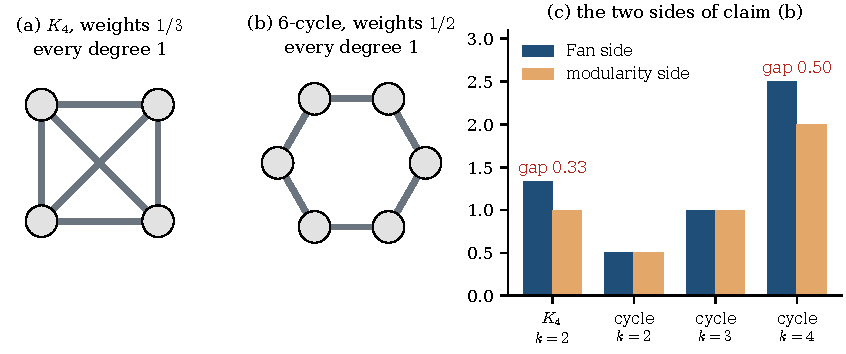
\includegraphics[width=\textwidth]{fig08_counterexamples.pdf}
\caption{Two unit-degree counterexamples to (b) without its condition. (a) The complete
graph on 4 nodes with weights $1/3$ has $\lambda_2=4/3>1$: it fails already at $k=2$.
(b) The 6-cycle with weights $1/2$ has
$\operatorname{spec}(\Lap)=\{0,0.5,0.5,1.5,1.5,2\}$: it satisfies (b) for $k=2,3$ and
fails at $k=4$, where $\lambda_4=1.5$. (c) The Fan side
$\sum_{i\le k}\lambda_i$ against the modularity side $(k-1)-\sum_{i<k}\mu_i$; where
they differ, the gap is exactly $\lambda_k-1$.}
\label{fig:cex}
\end{figure}

\begin{remark}
Claim (c) inherits the same cut-off: $\max\{0,1-\lambda_2\}$ is 0 for every graph with
$\lambda_2\ge1$, so on such graphs it carries no information. This matters for the
time-varying graphs in Section~\ref{sec:scope}.
\end{remark}

\subsection{When do the Laplacian and modularity agree in general?}\label{sec:classify}

For general degrees, $\Bmat=\Dmat-\Lap-\dvec\dvec^\top/2m$. Each matrix has a direction it
treats as uninformative: $\Lap$ ignores $\one$ (everything moving together), while the
null term of $\Bmat$ points along $\dvec$ (each node moving in proportion to its degree).
The two share eigenvectors when the diagonal part is a multiple of the identity and the
two uninformative directions agree (Table~\ref{tab:classify}).

\begin{table}[htbp]
\centering\small\setlength{\tabcolsep}{4pt}
\begin{tabular}{lccc}
\toprule
setting & ignored by $\Lap$ & ignored by $\Bmat$ & same eigenvectors? \\
\midrule
regular, all degrees $c$ (includes unit degree) & $\one$ & $\one$ &
  yes: $\Bmat=c\Imat-\Lap-\tfrac cp\one\one^\top$ \\
normalised pair, any degrees & $\sqrt{\dvec}$ & $\sqrt{\dvec}$ &
  yes: $\Bmat_n=\Imat-\Lsym-\uvec\uvec^\top$ \\
plain pair, unequal degrees & $\one$ & $\dvec$ & no \\
\bottomrule
\end{tabular}
\caption{Three settings; $\uvec=\sqrt{\dvec/2m}$. The normalised identity is the
8 September result, and Part I is its special case $\dvec=\one$.}
\label{tab:classify}
\end{table}

\textbf{Regular.} If $\dvec=c\one$ then $\dvec\dvec^\top/2m=\tfrac cp\one\one^\top$ and the
proof of Lemma~\ref{lem:core} goes through with 1 replaced by $c$:
$\operatorname{spec}(\Bmat)=\{0\}\cup\{c-\lambda_i\}$.

\textbf{Normalised.} For any positive degrees, since $\Dmat^{-1/2}\dvec=\sqrt{\dvec}$,
$\Bmat_n=\Dmat^{-1/2}\Wmat\Dmat^{-1/2}-\uvec\uvec^\top=\Imat-\Lsym-\uvec\uvec^\top$, and
$\Lsym\uvec=\mathbf0$. Lemma~\ref{lem:core} applies verbatim with $\uvec$ in place of
$\one/\sqrt p$. So claim (a) holds for the normalised pair \emph{whatever the degrees}.

\textbf{Unequal degrees.} For an eigenvector $\vvec$ of $\Lap$,
$\Bmat\vvec=\Dmat\vvec-\lambda\vvec-\dvec(\dvec^\top\vvec)/2m$, which is not a multiple of
$\vvec$ in general. Figure~\ref{fig:degrees} shows the smallest example I found.

\begin{figure}[htbp]
\centering
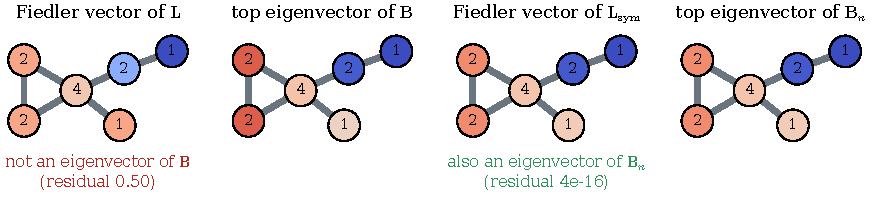
\includegraphics[width=\textwidth]{fig09_degrees.pdf}
\caption{A triangle with two tails; numbers are degrees, colours are eigenvector
entries. The Fiedler vector of $\Lap$ is not an eigenvector of $\Bmat$ (residual
$\lVert\Bmat\vvec-(\vvec^\top\Bmat\vvec)\vvec\rVert=0.50$), while the normalised pair
matches to $4.0\times10^{-16}$. On a graph this small the sign pattern, and so the split,
is still the same: different eigenvectors do not automatically mean different
clusters.}
\label{fig:degrees}
\end{figure}

\begin{aside}{Normalisation is not a free fix}
Normalising changes coordinates, not the graph, but it changes the statistical model:
Paper 1 uses $\Lap$ itself as the precision matrix, and using $\Lsym$ there would be a
different model. Inside Paper 1's framework, the only place modularity could add
information is the plain pair with unequal degrees, that is, after dropping the
unit-degree rule (Part III).
\end{aside}

\subsection{The check on Paper 1's learned graph}\label{sec:fig2}

The test case is Algorithm 1 on the S\&P data, the graph behind Paper 1's Fig.~2
(Figure~\ref{fig:fig2graph}). Its three components have 52, 28 and 17 stocks and are
exactly the three sectors (ARI 1.000). Because the degree rule is a penalty, the learned
degrees lie in $[1.0012,\,1.0069]$ rather than at exactly 1, so every prediction of
Proposition~\ref{prop:lemma} should hold approximately, with an error on the scale of
that tolerance. Table~\ref{tab:fig2} and Figure~\ref{fig:reflection} compare them.

\begin{figure}[htbp]
\centering
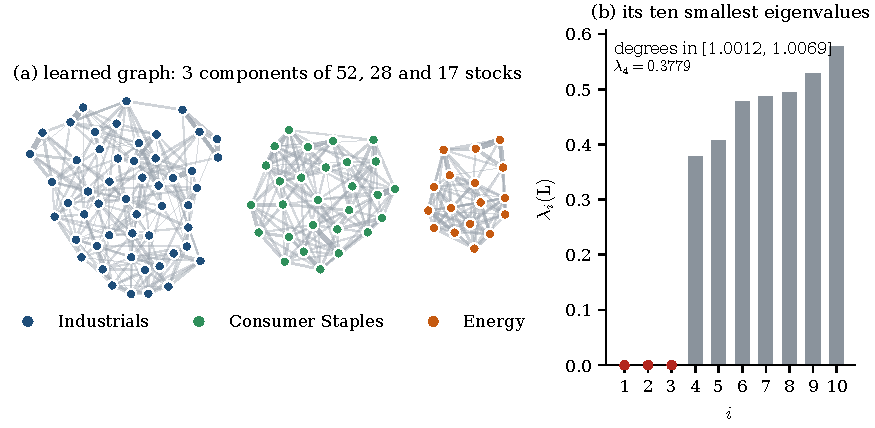
\includegraphics[width=\textwidth]{fig06_fig2_graph.pdf}
\caption{(a) The graph learned by Algorithm 1 from the S\&P data, coloured by sector;
edge width is weight, and the strongest 450 of its 1{,}194 edges are drawn. Each
component is exactly one sector. (b) Its Laplacian has three zero eigenvalues (one per
component) and then a gap.}
\label{fig:fig2graph}
\end{figure}

\begin{table}[htbp]
\centering\small
\begin{tabular}{>{\raggedright\arraybackslash}p{6.0cm}>{\raggedright\arraybackslash}p{2.6cm}>{\raggedright\arraybackslash}p{6.2cm}}
\toprule
quantity & Part I predicts & learned graph \\
\midrule
degrees $d_i$ & all 1 & in $[1.0012,\,1.0069]$, mean $1.0047$ \\
$\lVert\Bmat-(\Imat-\Lap-\one\one^\top/p)\rVert_F$ & 0 & $0.0479$ ($1.7\%$ of $\lVert\Bmat\rVert_F$) \\
three smallest $\lambda_i(\Lap)$ & 0, 0, 0 & all below $1.3\times10^{-15}$; next $0.3779$ \\
largest $\mu_i(\Bmat)$, claim (a) & 1, 1, then $1-\lambda_4$ & $1.0052$, $1.0041$, then $0.6274$ \\
claim (b): $\sum_{i\le3}\lambda_i$ against $2-\mu_1-\mu_2$ & equal & $6.7\times10^{-16}$ against $-0.0093$ \\
largest $|\lambda_i-(1-\mu_i)|$ over the 96 pairs & 0 & $0.0059$ (mean $0.0047$) \\
same, reflecting about the mean degree & 0 & $0.0020$ (mean $0.0006$) \\
$k$-means on the top 2 eigenvectors of $\Bmat$ & the components & ARI 1.000 against components and against sectors \\
\bottomrule
\end{tabular}
\caption{Part I's predictions on the learned graph. ``Reflecting about the mean degree''
uses the regular form of Table~\ref{tab:classify} with $c=\bar d=1.0047$.}
\label{tab:fig2}
\end{table}

\begin{figure}[htbp]
\centering
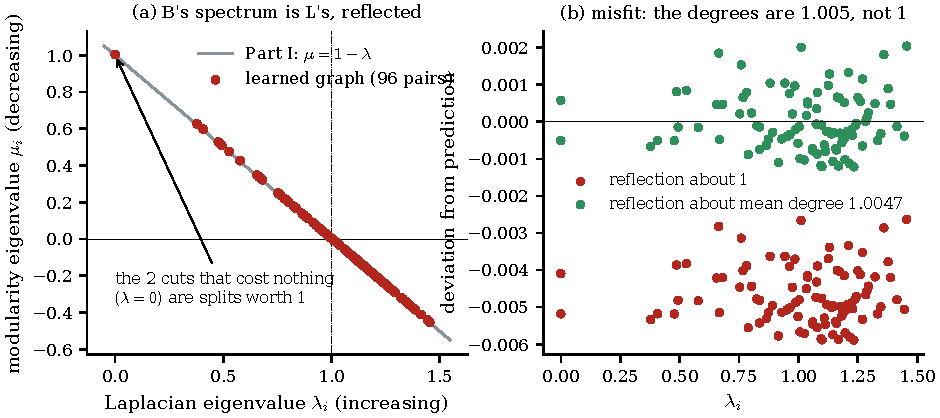
\includegraphics[width=\textwidth]{fig07_reflection.pdf}
\caption{(a) Each eigenvalue pair of the learned graph (on the directions orthogonal to
$\one$) lies on the line $\mu=1-\lambda$, as Lemma~\ref{lem:core} predicts. (b) The
remaining misfit, magnified. Reflecting about 1 leaves a uniform offset of about
$-0.005$ (red); reflecting about the mean degree $1.0047$ removes it (green), leaving
only the spread of the degrees around their mean.}
\label{fig:reflection}
\end{figure}

\textbf{Verdict: reproduced, within the solver's tolerance.} The partition prediction
holds exactly, and the spectral predictions hold to within the degree deviation. Most of
that deviation is a uniform shift: every degree is slightly above 1, so the graph is
closer to $c$-regular with $c=1.0047$ than to unit degree. This also explains why
$\mu_1,\mu_2$ slightly exceed the ceiling of 1 in (a), and why (b) misses by
$-0.0093\approx2(1-\bar d)$.

\subsection{Loosening the degree rule}\label{sec:sweep}

To see the identity fail as degrees spread, I reran Algorithm 1 on the same data with the
same settings, lowering only the degree penalty $\rho$. Every run still returns three
components and no isolated stock (Figure~\ref{fig:sweepgraphs}).

\begin{figure}[htbp]
\centering
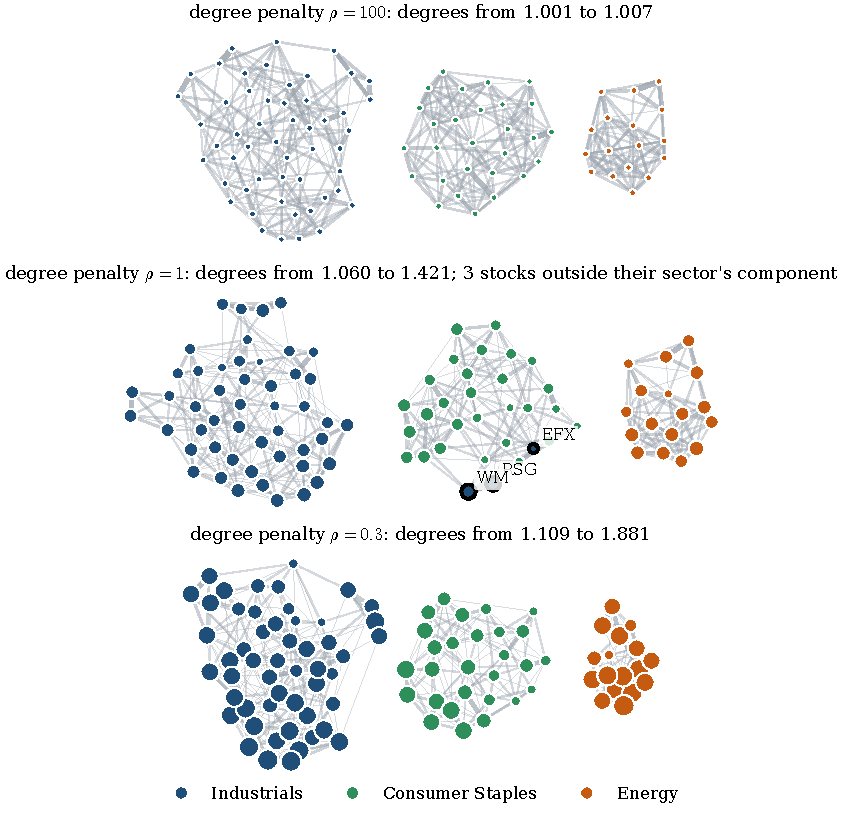
\includegraphics[width=0.93\textwidth]{fig10_sweep_graphs.pdf}
\caption{Algorithm 1 at three strengths of the degree rule; node size grows with
degree. At $\rho=100$ every degree is essentially 1. At $\rho=0.3$ they range up to
1.881, yet the components are still the sectors. At $\rho=1$ three Industrials stocks
(outlined: EFX, RSG and WM) join the Consumer Staples component.}
\label{fig:sweepgraphs}
\end{figure}

\begin{table}[htbp]
\centering\footnotesize\setlength{\tabcolsep}{3.5pt}
\begin{tabular}{rcccccccc}
\toprule
$\rho$ & degree range & degree CV & components & rel.\ residual & $\mu_1,\mu_2$ of $\Bmat$ & $\sin$ & ARI vs comp.\ & $\mu_1,\mu_2$ of $\Bmat_n$ \\
\midrule
100 & [1.001, 1.007] & 0.0014 & 52/28/17 & 0.017 & 1.005, 1.004 & 0.002 & 1.000 & 1, 1 \\
30  & [1.004, 1.023] & 0.0047 & 52/28/17 & 0.056 & 1.017, 1.013 & 0.008 & 1.000 & 1, 1 \\
10  & [1.011, 1.064] & 0.0129 & 52/28/17 & 0.152 & 1.048, 1.038 & 0.021 & 1.000 & 1, 1 \\
3   & [1.031, 1.184] & 0.0344 & 52/28/17 & 0.392 & 1.139, 1.110 & 0.058 & 1.000 & 1, 1 \\
1   & [1.060, 1.421] & 0.0700 & 49/31/17 & 0.730 & 1.318, 1.254 & 0.123 & 1.000 & 1, 1 \\
0.3 & [1.109, 1.881] & 0.1265 & 52/28/17 & 1.098 & 1.647, 1.491 & 0.236 & 1.000 & 1, 1 \\
\bottomrule
\end{tabular}
\caption{The sweep. Degree CV is the coefficient of variation (standard deviation over
mean) of the degrees. Relative residual is
$\lVert\Bmat-(\Imat-\Lap-\one\one^\top/p)\rVert_F/\lVert\Bmat\rVert_F$. $\sin$ is the
largest principal angle between the zero-eigenspace of $\Lap$ and the span of $\one$ and
the top two eigenvectors of $\Bmat$ (0 means the same subspace). ARI compares $k$-means
on the top two eigenvectors of $\Bmat$ with the components. The eigenvalues of $\Bmat_n$
equal 1 to six decimals in every row.}
\label{tab:sweep}
\end{table}

\begin{figure}[htbp]
\centering
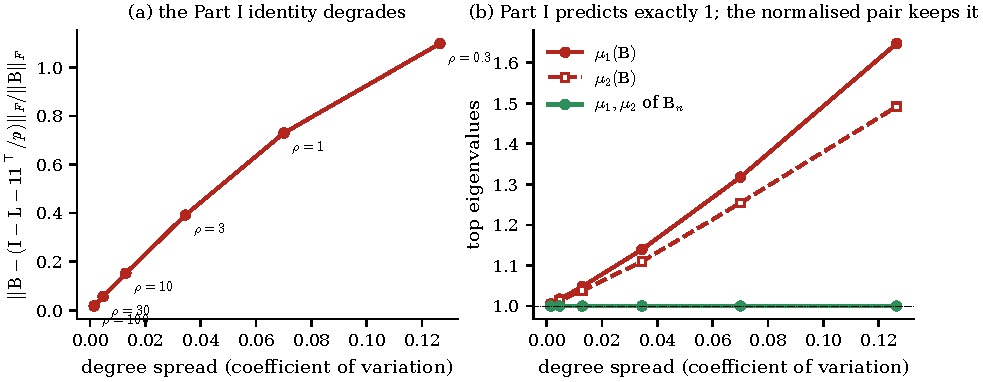
\includegraphics[width=\textwidth]{fig11_sweep_lines.pdf}
\caption{The sweep as degree spread grows. (a) The Part I identity degrades steadily,
reaching a residual larger than $\Bmat$ itself. (b) Part I predicts the top two
eigenvalues of $\Bmat$ are exactly 1; they climb to $1.65$. The normalised pair keeps
them at exactly 1 throughout.}
\label{fig:sweeplines}
\end{figure}

Three findings:
\begin{itemize}
\item \textbf{The algebra of Part I degrades steadily} as degrees spread (degree CV
  from $0.0014$ to $0.126$): the residual grows from $1.7\%$ to more than the size of
  $\Bmat$, and the top eigenvalues of $\Bmat$ pass the ceiling of 1 in (a).
\item \textbf{The normalised identity does not degrade at all}: $\Bmat_n$ keeps
  eigenvalue 1 exactly twice at every $\rho$, as Table~\ref{tab:classify} predicts.
\item \textbf{The partition survives}: even at $\rho=0.3$, $k$-means on the plain
  $\Bmat$ returns the components exactly. With three components and no edges between
  them, the eigenvector drift ($\sin\le0.24$) is too small to move any stock. I have no
  proof that this always happens.
\end{itemize}
The $\rho=1$ run is out of line: EFX, RSG and WM join Consumer Staples (ARI against
sectors 0.896). RSG and WM are waste-management companies and EFX a credit bureau, all
commonly treated as defensive, so the grouping is plausible; the runs on either side
return the sectors exactly. This is a property of that learned graph; the Part I
comparison still matches its components exactly.

\subsection{Where claim (c) applies}\label{sec:scope}

Claim (c) is exact under unit degree, but Paper 1's stress indicator comes from its
time-varying learner (its Problem (11)), which has no degree rule. Our 243 rolling-window
graphs for the FAAMUNG stocks (18 October note) have mean degree 2.13 and degree CV
0.305, more than twice the largest spread in Table~\ref{tab:sweep}, and $\lambda_2\ge1$
in 58\% of windows (140 of 243), where $\max\{0,1-\lambda_2\}$ is 0. On those graphs
$\mu_1$ and $\lambda_2$ are different quantities, so (c) does not connect the trading
indicator to modularity. If a modularity indicator on the time-varying graphs is still of
interest, the normalised identity $\mu_1(\Bmat_n)=\max\{0,1-\lambda_2(\Lsym)\}$ holds for
any degrees and could be the version to test.

\subsection{Part I conclusions}

Under the unit-degree rule the modularity matrix is a reflection of the Laplacian, so it
can neither find different clusters nor count them differently, and Algorithm 1's Fan
term is already a relaxed modularity. Paper 1's learned graph confirms this to within
the solver's tolerance. Modularity could only add information once degrees are allowed
to differ, which is Part III's direction; and the choice of null model, which is
Part II.

% =====================================================================
\section{Part II: the market as a built-in null model}\label{sec:part2}
% =====================================================================

\subsection{The question}

On most days the whole market rises or falls together. That shared movement explains a
large part of every stock's return, and it says nothing about which stocks belong
together; it is why nearly every entry of $\Smat$ is positive
(Figure~\ref{fig:data}). Modularity-based methods for correlation matrices therefore
subtract an explicit model of it before looking for groups. Paper 1 never does, yet it
recovers the sectors. Part II asks why, and whether it is always safe.

\begin{defn}{One-factor model, beta and loading}
The \emph{one-factor (market) model} writes each return as
$x_{t,i}=b_if_t+(\text{sector part})+(\text{noise})$, where $f_t$ is the market's return
on day $t$. The \emph{beta} $b_i$ says how strongly stock $i$ follows the market: 1 is
average, above 1 amplifies the market, below 1 dampens it. In a correlation matrix the
relevant quantity is the \emph{market loading} $b_i=\operatorname{corr}(x_i,f)$; I use
both, and call both ``beta'' where the difference does not matter. Here the market is
the S\&P 500 index (\texttt{\^{}GSPC}).
\end{defn}

\subsection{The learner removes the market on its own}\label{sec:implicit}

Let $\Jmat=\Imat-\one\one^\top/p$. Applying $\Jmat$ to a vector subtracts its average, so
$\Jmat\Smat\Jmat$ is the correlation structure of the returns after \emph{each day's
average across stocks} has been removed.

\begin{proposition}\label{prop:implicit}
For every Laplacian $\Lap$ and every symmetric $\Smat$,
$\tr(\Lap\Smat)=\tr(\Lap\Jmat\Smat\Jmat)$. Hence Problem (1), Algorithm 1 and any learner
whose only data term is $\tr(\Lap\Smat)$ learn the same graph from $\Smat$ and from
$\Jmat\Smat\Jmat$.
\end{proposition}
\begin{proof}
$\Lap\one=\mathbf0$ gives $\Lap\Jmat=\Lap$ and, by symmetry, $\Jmat\Lap=\Lap$. So
$\tr(\Lap\Jmat\Smat\Jmat)=\tr(\Jmat\Lap\Jmat\Smat)=\tr(\Lap\Smat)$. The other terms of the
objectives depend on $\Lap$ alone.
\end{proof}

So the learner works with the de-averaged data whether we ask it to or not. What does
that remove? Take the one-factor model, $\Smat=\sigma^2\bvec\bvec^\top+\Smat_0$, with
$\Smat_0$ the sector and noise parts. By \eqref{eq:quad}, the market's share of the data
fit is
\begin{equation}\label{eq:market}
  \tr(\Lap\,\sigma^2\bvec\bvec^\top)=\sigma^2\,\bvec^\top\Lap\bvec=\sigma^2\sum_{i<j}W_{ij}(b_i-b_j)^2 .
\end{equation}

\begin{itemize}
\item \textbf{Equal betas are removed exactly.} If every $b_i$ is the same, \eqref{eq:market}
  is 0 for every graph: the learner ignores the market completely, with no model of it.
\item \textbf{Unequal betas leave a penalty.} Otherwise each link pays in proportion to
  the squared beta difference of its two stocks, so the learner is pushed to link
  stocks with similar betas. Equivalently, it sees $\sigma^2(\Jmat\bvec)(\Jmat\bvec)^\top$,
  which acts like an extra factor sorting stocks by beta.
\end{itemize}

\begin{defn}{Beta inequality $\sin^2\theta$}
The total size of the penalty over all pairs is
\[
  \sum_{i<j}(b_i-b_j)^2=p\sum_ib_i^2-\Big(\sum_ib_i\Big)^2=p\lVert\Jmat\bvec\rVert^2
  =p\lVert\bvec\rVert^2\sin^2\theta,\qquad
  \sin^2\theta=1-\frac{(\one^\top\bvec)^2}{p\lVert\bvec\rVert^2},
\]
where $\theta$ is the angle between the beta vector and $\one$. $\sin^2\theta$ is 0 when
all betas are equal and grows as they spread; it does not depend on the overall size of
the betas. It is the measure of beta inequality used throughout Part II.
\end{defn}

Whether the penalty helps or hurts depends on where the betas sit relative to the
groups. If stocks in the same sector have similar betas, the penalty falls on links
between sectors and \emph{reinforces} the sectors. If betas vary inside sectors, it
\emph{competes} with them.

\begin{defn}{Explicit nulls compared}
Four standard ways to remove the market before learning, plus one available only in
simulation:
\begin{enumerate}[label=(\roman*)]
\item \emph{S-mode}: subtract the top eigenvector component $\mu_1\uvec_1\uvec_1^\top$ of
  $\Smat$ (the ``market mode''), then rescale to unit diagonal;
\item \emph{resid-SPX}: regress each stock on the S\&P 500 index and use the
  correlation of the residuals;
\item \emph{resid-EW}: the same, on the equal-weighted average of the 97 stocks;
\item \emph{RMT}: the ``group component'' of MacMahon and Garlaschelli (2015). Random
  matrix theory says that for pure noise the eigenvalues of a correlation matrix stay
  below the \emph{Marchenko-Pastur edge} $(1+\sqrt{p/T})^2$; the group component keeps
  only the eigenvalue modes above that edge, minus the market mode;
\item \emph{oracle} (simulation only): residuals on the true market factor.
\end{enumerate}
\end{defn}

\subsection{Real data: the S\&P panel}\label{sec:real}

The loadings of the 97 stocks on the S\&P 500 lie in $[0.177,\,0.743]$ (mean $0.513$),
so $\sin^2\theta=0.064$; the regression betas lie in $[0.347,\,1.839]$. The betas are
largely a property of the sector: mean loadings are 0.363 for Consumer Staples, 0.597 for
Industrials and 0.506 for Energy (mean regression betas 0.568, 1.042 and 1.192), and
$57.7\%$ of the variation in loadings is between sectors rather than within them
(Figure~\ref{fig:marketreal}). For the RMT null the Marchenko-Pastur edge is $1.847$, and
4 group modes lie above it.

\begin{figure}[htbp]
\centering
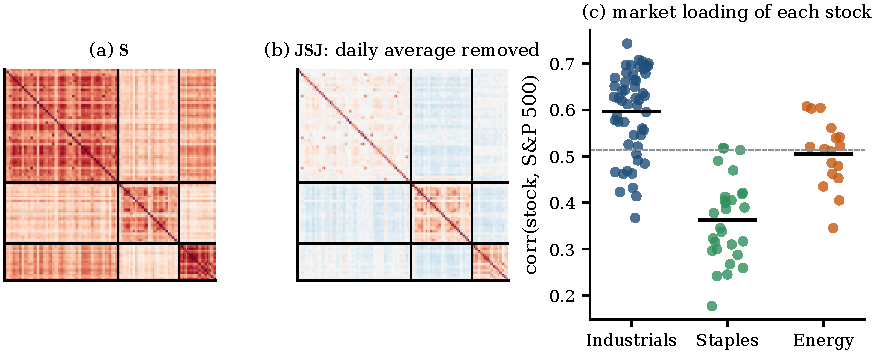
\includegraphics[width=\textwidth]{fig12_market_real.pdf}
\caption{(a) The correlation matrix, sorted by sector. (b) After removing each day's
average ($\Jmat\Smat\Jmat$), the uniform positive background is gone and the sector blocks
stand out; this is what the learner actually sees. (c) Each stock's loading on the
S\&P 500, by sector (bars: sector means; dashed: overall mean). Consumer Staples are
defensive, low-beta stocks.}
\label{fig:marketreal}
\end{figure}

Table~\ref{tab:real} runs both learners on all six inputs. Besides the ARI, it reports a
\emph{beta ratio}: the link-weighted average of $|b_i-b_j|$ over same-sector pairs,
divided by the plain average over the same pairs. Values below 1 mean that within a
sector the graph prefers to link stocks with similar betas, which is the penalty
\eqref{eq:market} at work.

\begin{table}[htbp]
\centering\small\setlength{\tabcolsep}{4.5pt}
\begin{tabular}{lccccccc}
\toprule
 & \multicolumn{4}{c}{Algorithm 1 ($k=3$)} & \multicolumn{3}{c}{Problem (1) + $k$-means} \\
\cmidrule(lr){2-5}\cmidrule(lr){6-8}
input & comp. & ARI sectors & ARI beta & beta ratio & ARI sectors & ARI beta & beta ratio \\
\midrule
$\Smat$ (built-in null) & 3 & \textbf{1.000} & 0.277 & 0.786 & \textbf{0.900} & 0.295 & 0.862 \\
$\Jmat\Smat\Jmat$ & 3 & 1.000 & 0.277 & 0.786 & 0.900 & 0.295 & 0.862 \\
\midrule
S-mode & 1 & 0.830 & 0.257 & 0.820 & 0.867 & 0.292 & 0.879 \\
resid-SPX & 1 & 0.830 & 0.257 & 0.816 & 0.802 & 0.252 & 0.872 \\
resid-EW & 3 & 0.896 & 0.298 & 0.794 & 0.867 & 0.292 & 0.867 \\
RMT & 1 & 0.875 & 0.291 & 0.928 & 0.900 & 0.268 & 0.944 \\
\bottomrule
\end{tabular}
\caption{The S\&P panel. ``comp.'' is the number of components Algorithm 1 returns;
where it is 1, clusters come from $k$-means on the bottom three eigenvectors. ARI beta
compares the clusters with a three-way split of the stocks by loading.}
\label{tab:real}
\end{table}

\begin{figure}[htbp]
\centering
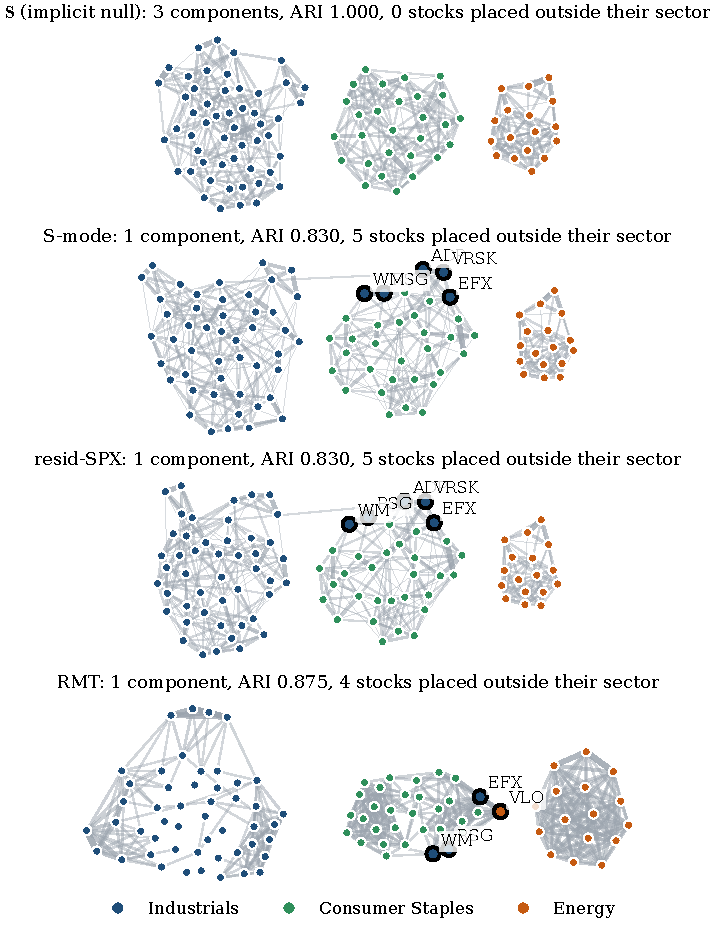
\includegraphics[width=0.92\textwidth]{fig13_real_graphs.pdf}
\caption{Algorithm 1's graphs from four of the inputs, coloured by sector, drawn with
each detected cluster laid out separately. Outlined and labelled: stocks placed in a
cluster dominated by another sector. The built-in null gets every stock right; the
explicit nulls move the same handful of Industrials stocks into Consumer Staples (and,
for RMT, the refiner VLO).}
\label{fig:realgraphs}
\end{figure}

\begin{itemize}
\item \textbf{The invariance holds numerically.} Graphs from $\Smat$ and from
  $\Jmat\Smat\Jmat$ agree to $2.7\times10^{-10}$ (Problem (1)) and $1.3\times10^{-4}$
  (Algorithm 1, within its stopping tolerance), and every metric is identical.
\item \textbf{No explicit null beats the built-in one.} Under Algorithm 1 every explicit
  null loses: ARI 0.830 to 0.896 against 1.000. Under Problem (1) the RMT null ties at
  0.900 and the rest lose (0.802 to 0.867). \emph{Explicit market removal improving on the
  built-in null: not supported on this data.}
\item \textbf{The same stocks move every time.} Apart from the refiner VLO, every
  misplaced stock is one of ADP, EFX, RSG, VRSK and WM (payroll, credit-data, analytics
  and waste-management companies: Industrials by classification, defensive by
  behaviour), and each joins Consumer Staples (Figure~\ref{fig:realgraphs}). VLO is
  misplaced by Problem (1) on every input, the built-in null included, and by
  Algorithm 1 on RMT.
\item \textbf{A likely reason: betas carry sector information here.} With $57.7\%$ of
  the loading variance between sectors, the penalty \eqref{eq:market} falls mostly on
  links between sectors and supports the sector split. Removing the market removes that
  support, and the low-beta Industrials stocks drift towards the low-beta sector.
\item \textbf{The penalty is visible inside sectors.} With the built-in null the beta
  ratio is 0.786 (Algorithm 1) and 0.862 (Problem (1)); every explicit null raises it,
  RMT the most (0.928, 0.944), as \eqref{eq:market} predicts once the market term is
  gone. In absolute terms the market term is small: $\bvec^\top\Lap\bvec$ is $1.1\%$ of
  $\tr(\Lap\Smat)$ on the Algorithm 1 graph and $1.7\%$ on the Problem (1) graph.
\end{itemize}

\subsection{Simulated markets: when betas cut across sectors}\label{sec:synthetic}

The S\&P data cannot show what happens when betas vary \emph{within} sectors, so I
simulated it.

\textbf{Model.} $x_{t,i}=b_if_t+s_{g(i),t}+e_{t,i}$, with a market factor
$f_t\sim N(0,1)$, one factor per sector $s_{g,t}\sim N(0,0.6^2)$ and noise
$e_{t,i}\sim N(0,1.2^2)$, all independent; $p=60$ stocks in three sectors of 20, and
$T=753$ days as in the real data. Three beta designs (Figure~\ref{fig:design}):
\emph{equal} (every $b_i=1$); \emph{aligned} ($b_i=1-\delta,\ 1,\ 1+\delta$ by sector);
and \emph{cross} (in every sector, half the stocks at $1+\delta$ and half at $1-\delta$).
The population loadings are $b_i/\sqrt{b_i^2+0.6^2+1.2^2}$, and $\sin^2\theta$ is
computed from them. Each simulated data set is learned from $\Smat$, from S-mode and
from the oracle, with both learners.

\begin{figure}[htbp]
\centering
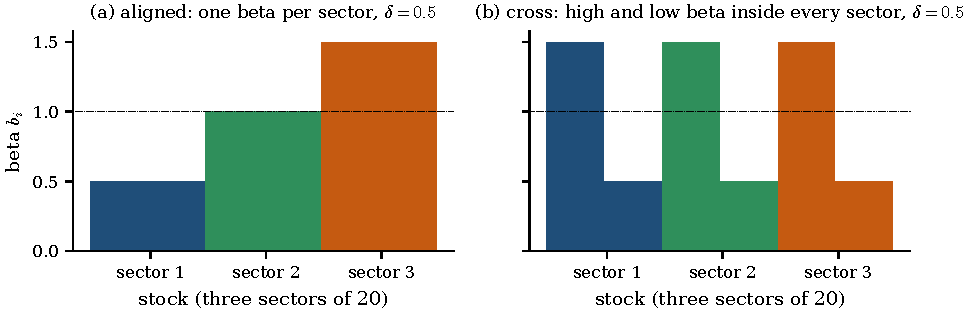
\includegraphics[width=\textwidth]{fig14_synthetic_design.pdf}
\caption{The two unequal-beta designs at $\delta=0.5$. (a) Aligned: betas follow the
sectors, as on the real data. (b) Cross: the beta split is orthogonal to the sectors,
so the penalty \eqref{eq:market} competes with them.}
\label{fig:design}
\end{figure}

\textbf{Coarse grid} ($\delta=0.2,0.4,0.6,0.8$, two seeds; 108 runs).
\begin{itemize}
\item \emph{Equal and aligned}: every input and learner recovers the sectors exactly
  (ARI 1.000) in every run, up to $\sin^2\theta=0.219$. Unequal betas are harmless when
  they follow the groups. This is the real-data situation.
\item \emph{Cross}: exact at $\delta=0.2$ and 0.4 ($\sin^2\theta=0.017$, 0.072). At
  $\delta=0.6$ and 0.8 ($\sin^2\theta=0.173$, 0.322) both learners on $\Smat$ cluster by
  beta in both seeds: ARI 0.134 against the sectors and 0.773 against the two beta
  groups (not 1, because there are three clusters for two groups). S-mode and the
  oracle stay at 1.000 (Figure~\ref{fig:syngraphs}).
\end{itemize}

\begin{figure}[htbp]
\centering
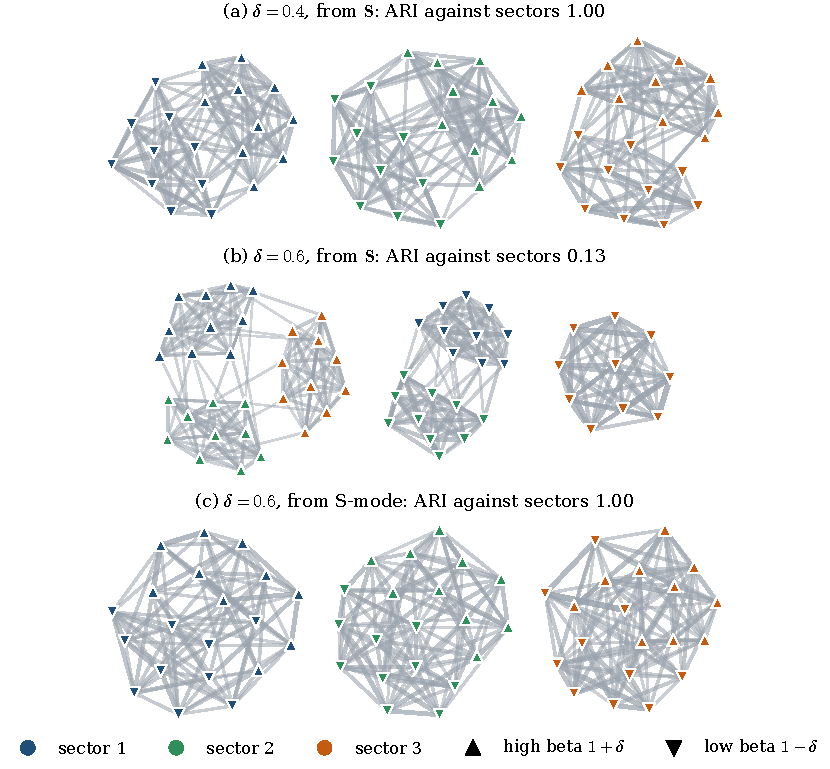
\includegraphics[width=0.88\textwidth]{fig15_synthetic_graphs.pdf}
\caption{Algorithm 1 on simulated cross-design data (seed 0). Colour is the true sector,
the triangle's direction the beta group. (a) At $\delta=0.4$ the components are the
sectors. (b) At $\delta=0.6$ they are held together by beta instead: one component holds all
30 high-beta stocks from every sector, and the low-beta stocks split in two. (c) The same
data with the market mode removed: the sectors again.}
\label{fig:syngraphs}
\end{figure}

\textbf{Fine grid} (cross design, $\delta$ from 0.400 to 0.600 in steps of 0.025, five
seeds; 270 runs). Table~\ref{tab:threshold} and Figure~\ref{fig:threshold} locate the
switch. S-mode and the oracle give ARI 1.000 in all 180 of their runs.

\begin{table}[htbp]
\centering\small
\begin{tabular}{cccccc}
\toprule
 & & \multicolumn{2}{c}{Algorithm 1 on $\Smat$} & \multicolumn{2}{c}{Problem (1) on $\Smat$} \\
\cmidrule(lr){3-4}\cmidrule(lr){5-6}
$\delta$ & $\sin^2\theta$ & ARI sectors & seeds by beta & ARI sectors & seeds by beta \\
\midrule
0.400 & 0.0715 & 1.000 & 0/5 & 1.000 & 0/5 \\
0.425 & 0.0815 & 1.000 & 0/5 & 1.000 & 0/5 \\
0.450 & 0.0921 & 1.000 & 0/5 & 1.000 & 0/5 \\
0.475 & 0.1036 & 1.000 & 0/5 & 1.000 & 0/5 \\
0.500 & 0.1158 & 1.000 & 0/5 & 0.767 & 1/5 \\
0.525 & 0.1288 & 1.000 & 0/5 & 0.346 & 3/5 \\
0.550 & 0.1426 & 0.767 & 1/5 & 0.134 & 5/5 \\
0.575 & 0.1572 & 0.459 & 2/5 & 0.134 & 5/5 \\
0.600 & 0.1726 & 0.134 & 5/5 & 0.134 & 5/5 \\
\bottomrule
\end{tabular}
\caption{The switch from sectors to beta groups, cross design. ARI is the mean over five
seeds; ``seeds by beta'' counts the seeds whose clusters match the beta groups better
than the sectors.}
\label{tab:threshold}
\end{table}

\begin{figure}[htbp]
\centering
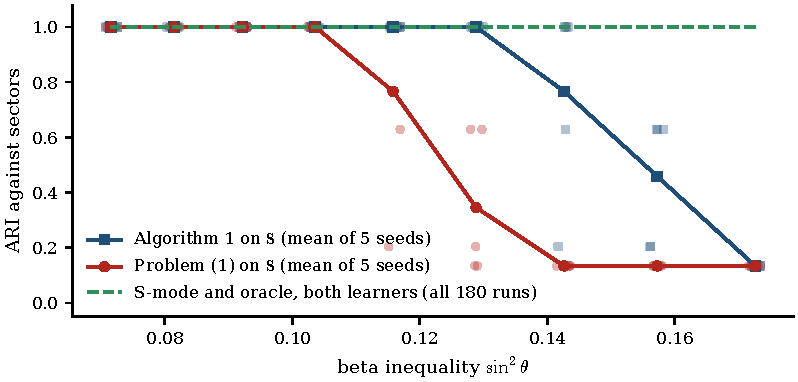
\includegraphics[width=0.85\textwidth]{fig16_threshold.pdf}
\caption{ARI against the sectors as beta inequality grows (cross design; faint markers
are single seeds, lines are means). The built-in null switches to clustering by beta
over a narrow range; the explicit nulls never do.}
\label{fig:threshold}
\end{figure}

The switch is sharp. For Problem (1) it begins between $\sin^2\theta=0.104$ and $0.116$
and is complete by $0.143$; for Algorithm 1 it begins between $0.129$ and $0.143$ and is
complete by $0.173$. Algorithm 1 holds out longer; I have not tested why. Where the
switch happens depends on how strong the sector factor is relative to the noise, which
here is our choice ($0.6$ against $1.2$). So these values belong to this design, and the
real data's $\sin^2\theta=0.064$ cannot be compared with them directly.
Section~\ref{sec:boundcheck} gives a comparison that does carry over.

\subsection{A perturbation bound}\label{sec:bound}

The proposal asks for a bound that links beta inequality to how far the cluster
eigenvectors can move. I derive it for Problem (1), which is convex; Algorithm 1 is not,
and the argument does not apply to it. Two more terms are needed.

\begin{defn}{Principal angles and $\lVert\sin\Theta\rVert_F$}
To compare two $k$-dimensional subspaces (here, the spans of the bottom $k$ eigenvectors
of two Laplacians), one uses their $k$ \emph{principal angles} $\theta_1,\dots,\theta_k$:
the smallest angles that can be achieved between unit vectors, one from each subspace,
chosen one pair at a time. $\lVert\sin\Theta\rVert_F=(\sum_i\sin^2\theta_i)^{1/2}$ is 0
for identical subspaces and at most $\sqrt k$.
\end{defn}
\begin{defn}{Strong convexity and the Davis-Kahan theorem}
A function is \emph{$\mu$-strongly convex} if its curvature is at least $\mu$ in every
direction; then a small change in its linear part can move the minimiser only a little.
The \emph{Davis-Kahan theorem} is the classic statement that the eigenvectors of a
symmetric matrix move little under a perturbation that is small compared with the
eigengap separating them from the others.
\end{defn}

In the edge weights $\wvec=(W_{ij})_{i<j}\ge0$, Problem (1) reads
$\min_{\wvec\ge0}\langle\wvec,\zvec(\Smat)+\beta\one\rangle+g(\wvec)$, with
$z_{ij}=S_{ii}+S_{jj}-2S_{ij}$ and $g(\wvec)=-\log\gdet\Lap(\wvec)$. Adding the market
term $\bvec\bvec^\top$ to $\Smat$ adds $\Delta z_{ij}=(b_i-b_j)^2$ to $\zvec$: a linear
change, of total size $\lVert\Delta\zvec\rVert_1=p\lVert\bvec\rVert^2\sin^2\theta$. Let
$\wvec_c$ solve the clean problem (from $\Smat-\bvec\bvec^\top$) and $\wvec_o$ the
observed one (from $\Smat$).

\begin{proposition}[Step 1]\label{prop:step1}
Suppose both solutions are connected graphs and let $M$ be the larger of their largest
Laplacian eigenvalues. Then
\[
  \langle\Delta\zvec,\wvec_o-\wvec_c\rangle\le0,\qquad
  \lVert\wvec_o-\wvec_c\rVert\le\frac{M^2}{2}\lVert\Delta\zvec\rVert,\qquad
  \lVert\Lap(\wvec_o)-\Lap(\wvec_c)\rVert_F\le\sqrt{2p}\,\lVert\wvec_o-\wvec_c\rVert .
\]
\end{proposition}
\begin{proof}
\emph{Curvature.} For a connected $\Lap$ and a direction $\mathbf h$, the second
derivative of $g$ is $\tr(\Lap^+\Lap(\mathbf h)\Lap^+\Lap(\mathbf h))$, with $\Lap^+$ the
pseudo-inverse. $\Lap(\mathbf h)$ acts on the directions orthogonal to $\one$, where
$\Lap^+\succeq\lambda_{\max}^{-1}\Imat$, so the second derivative is at least
$\lVert\Lap(\mathbf h)\rVert_F^2/\lambda_{\max}^2$, and
$\lVert\Lap(\mathbf h)\rVert_F^2=\sum_i(\sum_jh_{ij})^2+2\lVert\mathbf h\rVert^2\ge
2\lVert\mathbf h\rVert^2$. Every graph on the segment between $\wvec_c$ and $\wvec_o$ is
connected and, since $\lambda_{\max}$ is convex in $\wvec$, has $\lambda_{\max}\le M$.
So $g$ is $\mu$-strongly convex there with $\mu=2/M^2$.

\emph{Comparison.} Optimality over $\wvec\ge0$ gives
$\langle\zvec+\Delta\zvec+\beta\one+\nabla g(\wvec_o),\wvec_c-\wvec_o\rangle\ge0$ and
$\langle\zvec+\beta\one+\nabla g(\wvec_c),\wvec_o-\wvec_c\rangle\ge0$. Adding them,
\[
  \mu\lVert\wvec_o-\wvec_c\rVert^2\le\langle\nabla g(\wvec_o)-\nabla g(\wvec_c),\wvec_o-\wvec_c\rangle
  \le\langle\Delta\zvec,\wvec_c-\wvec_o\rangle\le\lVert\Delta\zvec\rVert\,\lVert\wvec_o-\wvec_c\rVert .
\]
The middle inequality gives the sign statement, and dividing gives the second claim.
For the third, Cauchy-Schwarz gives $(\sum_jh_{ij})^2\le(p-1)\sum_jh_{ij}^2$; summing
over $i$ and adding $2\lVert\mathbf h\rVert^2$ gives at most $2p\lVert\mathbf h\rVert^2$.
\end{proof}

The sign statement reads plainly: compared with the clean graph, the observed graph has,
in aggregate, moved weight away from pairs with different betas.

\textbf{Step 2} is the Davis-Kahan theorem in the form of Yu, Wang and Samworth (2015,
Theorem 2). With $\mathrm{gap}=\lambda_{k+1}(\Lap_c)-\lambda_k(\Lap_c)>0$, the bottom-$k$
eigenvector subspaces satisfy
$\lVert\sin\Theta\rVert_F\le2\sqrt k\,\lVert\Delta\Lap\rVert_2/\mathrm{gap}$, where
$\lVert\cdot\rVert_2$ is the largest singular value. Chaining both steps through
$\lVert\Delta\Lap\rVert_2\le\lVert\Delta\Lap\rVert_F$,
\begin{equation}\label{eq:chain}
  \lVert\sin\Theta\rVert_F\le\frac{\sqrt{2kp}\,M^2\,\lVert\Delta\zvec\rVert}{\mathrm{gap}},
  \qquad\lVert\Delta\zvec\rVert\le p\lVert\bvec\rVert^2\sin^2\theta .
\end{equation}
This is the shape the proposal anticipated: the cluster subspace moves by at most a
constant times $\sin^2\theta/\mathrm{gap}$. Since $\lVert\sin\Theta\rVert_F\le\sqrt k$
always, \eqref{eq:chain} only says something when its right side is below $\sqrt k$.

\subsection{The bound against the measurements}\label{sec:boundcheck}

Table~\ref{tab:bound} evaluates each step for Problem (1) on the cross design (mean over
three seeds) and on the real data. The clean graph is learned from
$\Smat-\bvec\bvec^\top$, using the population loadings (simulation) or the sample loadings
on the S\&P 500 (real). $M$ is between 0.189 and 0.195 in every row.

\begin{table}[htbp]
\centering\footnotesize\setlength{\tabcolsep}{3pt}
\begin{tabular}{ccccccccccccc}
\toprule
 & & \multicolumn{3}{c}{Step 1: $\lVert\Delta\wvec\rVert$} & \multicolumn{2}{c}{$\lVert\Delta\Lap\rVert$} & & & & \multicolumn{2}{c}{Step 2: DK} & \\
\cmidrule(lr){3-5}\cmidrule(lr){6-7}\cmidrule(lr){11-12}
$\delta$ & $\sin^2\theta$ & actual & bound & ratio & 2-norm & F bound & gap & $\dfrac{\lVert\Delta\Lap\rVert_2}{\mathrm{gap}}$ & $\lVert\sin\Theta\rVert_F$ & true $\Delta\Lap$ & chain & ARI \\
\midrule
0.20 & 0.017 & 0.0078 & 0.0129 & 1.65 & 0.0111 & 0.141 & 0.0451 & 0.247 & 0.007 & 0.86 & 10.9 & 1.00 \\
0.30 & 0.039 & 0.0164 & 0.0296 & 1.80 & 0.0234 & 0.324 & 0.0443 & 0.528 & 0.022 & 1.83 & 25.4 & 1.00 \\
0.40 & 0.072 & 0.0268 & 0.0540 & 2.02 & 0.0381 & 0.592 & 0.0435 & 0.877 & 0.070 & 3.04 & 47.2 & 1.00 \\
0.45 & 0.092 & 0.0322 & 0.0693 & 2.15 & 0.0459 & 0.759 & 0.0430 & 1.067 & 0.147 & 3.70 & 61.2 & 1.00 \\
0.50 & 0.116 & 0.0377 & 0.0868 & 2.30 & 0.0537 & 0.951 & 0.0425 & 1.263 & 0.375 & 4.38 & 77.6 & 0.73 \\
0.55 & 0.143 & 0.0431 & 0.1067 & 2.47 & 0.0614 & 1.169 & 0.0420 & 1.464 & 0.947 & 5.08 & 96.6 & 0.13 \\
0.60 & 0.173 & 0.0484 & 0.1290 & 2.67 & 0.0689 & 1.413 & 0.0413 & 1.668 & 0.984 & 5.78 & 118.6 & 0.13 \\
0.80 & 0.322 & 0.0673 & 0.2445 & 3.63 & 0.0957 & 2.678 & 0.0381 & 2.509 & 0.994 & 8.70 & 243.5 & 0.13 \\
\midrule
real & 0.064 & 0.0156 & 0.0756 & 4.84 & 0.0212 & 1.053 & 0.0317 & 0.669 & 0.157 & 2.32 & 114.9 & 0.90 \\
\bottomrule
\end{tabular}
\caption{Problem (1). ``ratio'' is the Step 1 bound over the actual movement; ``2-norm''
is the actual $\lVert\Delta\Lap\rVert_2$; ``F bound'' is $\sqrt{2p}$ times the Step 1
bound; ``true $\Delta\Lap$'' is the Davis-Kahan bound evaluated with the actual change;
``chain'' is \eqref{eq:chain}. Any Davis-Kahan value above $\sqrt k=1.732$ says nothing.
ARI is that of the observed graph against the sectors; the clean graph scores 1.00 in
every simulated row and 0.87 on the real data.}
\label{tab:bound}
\end{table}

\begin{figure}[htbp]
\centering
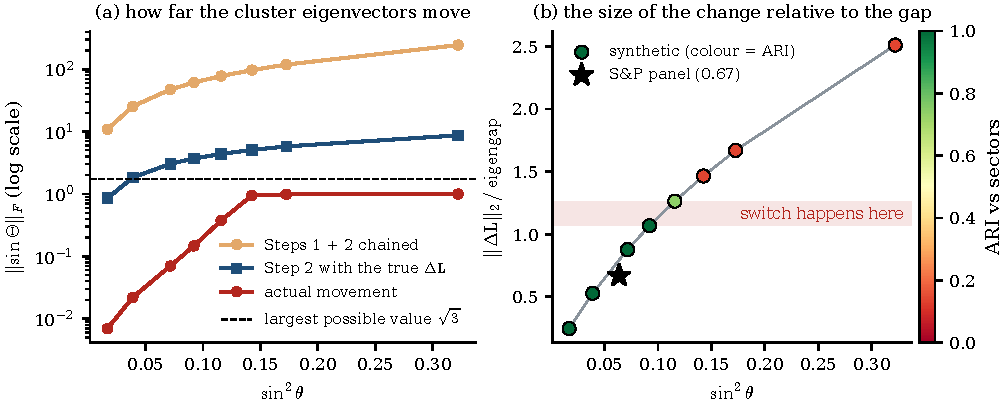
\includegraphics[width=\textwidth]{fig17_bound.pdf}
\caption{(a) How far the cluster eigenvectors actually move (red) against what the
bound allows, with the true change in the graph (blue) and fully chained (orange).
Everything above the dashed line is uninformative. (b) The change in the graph measured
in units of the eigengap. The switch to beta clusters happens between 1.067 and 1.263
(shaded); the real data sits at 0.669.}
\label{fig:bound}
\end{figure}

\begin{itemize}
\item \textbf{Step 1 is valid and fairly tight}: the bound on the weight change exceeds
  the actual change by a factor 1.65 to 3.63 in simulation (2.15 to 2.47 near the
  switch) and 4.84 on the real data. \emph{Reproduced.}
\item \textbf{Passing to $\Delta\Lap$ loses a further factor of about 8.} At
  $\delta=0.5$ the actual ratio $\lVert\Delta\Lap\rVert_F/\lVert\Delta\wvec\rVert$ is 1.43,
  against the worst case $\sqrt{2p}=10.95$: the weight changes are spread over many
  links and largely cancel in each node's total.
\item \textbf{Step 2 is uninformative here, even with the true $\Delta\Lap$.} The clean
  graph's eigengap is only about 0.04, so the Davis-Kahan bound passes $\sqrt k$ already
  at $\delta=0.3$, where the subspace has in fact moved by 0.022. The full chain gives
  10.9 to 243.5 against a ceiling of 1.732. \emph{Proved, but vacuous on this problem.}
\item \textbf{The ratio $\lVert\Delta\Lap\rVert_2/\mathrm{gap}$ does locate the switch.}
  At 0.877 and 1.067 nothing has switched ($\lVert\sin\Theta\rVert_F$ 0.070 and 0.147); at
  1.263 one seed in three has (0.375); at 1.464 all have (0.947). The switch happens when
  the change reaches roughly the eigengap, which is the scale Davis-Kahan identifies; its
  constant and the slack in Step 1 put the certified threshold far below the real one.
\item \textbf{On the real data the ratio is 0.669}, below every simulated row that
  switched. Unlike $\sin^2\theta$, this comparison does not depend on the sector
  strength, since the change and the gap are both measured on the data. It agrees with
  the finding that the built-in null suffices there. It is a measured rule on one design
  and one learner, not a theorem.
\end{itemize}

\subsection{Part II conclusions}

The Laplacian learner removes the market for free, exactly when betas are equal. When
betas differ, what is left is a penalty on linking stocks with different betas. On the
S\&P data that penalty helps, because betas follow sectors, and explicit removal of the
market makes clustering worse. When betas vary within sectors, the penalty can take
over, and does so abruptly; explicit removal then recovers the sectors. The proved
bound has the right form but constants far too loose to predict the switch; the
measured rule ``switch when the graph change reaches the eigengap'' does.

% =====================================================================
\section{Status, deviations and next steps}\label{sec:status}
% =====================================================================

\subsection{Status of every claim}

\begin{center}
\small
\renewcommand{\arraystretch}{1.2}
\begin{tabular}{>{\raggedright\arraybackslash}p{5.3cm}>{\raggedright\arraybackslash}p{2.7cm}>{\raggedright\arraybackslash}p{6.6cm}}
\toprule
claim & status & evidence \\
\midrule
\multicolumn{3}{l}{\textit{Part I}} \\
(a) components counted by eigenvalue 1 of $\Bmat$ & proved; reproduced & Prop.~\ref{prop:lemma}; learned graph gives $1.0052$, $1.0041$ (degree tolerance) \\
(b) Fan term $=$ relaxed modularity & proved; holds when $\lambda_k\le1$ & exact form with $\max\{0,\lambda_k-1\}$; two counterexamples; learned graph misses by $0.0093$ \\
(c) $\mu_1=\max\{0,1-\lambda_2\}$ & proved; unit degree only & does not apply to the time-varying graphs (Section~\ref{sec:scope}) \\
regular / normalised / unequal degrees & proved & Table~\ref{tab:classify}; $\Bmat_n$ exact in every sweep run \\
$k$-means on $\Bmat$ recovers the components & reproduced & ARI 1.000 on the learned graph and at every $\rho$ \\
\multicolumn{3}{l}{\textit{Part II}} \\
$\tr(\Lap\Smat)=\tr(\Lap\Jmat\Smat\Jmat)$ & proved; reproduced & graphs agree to $2.7\times10^{-10}$ and $1.3\times10^{-4}$ \\
market term is a beta-difference penalty, size $\propto\sin^2\theta$ & proved & \eqref{eq:market}; unit tests \\
built-in null suffices on the S\&P data & reproduced & Algorithm 1 ARI 1.000 \\
explicit null improves on it (real data) & \textbf{not supported} & Algorithm 1: 0.830 to 0.896; Problem (1): 0.802 to 0.900 \\
aligned unequal betas are harmless & reproduced (simulation) & ARI 1.000 in every aligned run \\
cross-cutting betas break the built-in null & reproduced (simulation) & switch at $\sin^2\theta$ 0.116 to 0.143 (Problem (1)), 0.143 to 0.173 (Algorithm 1) \\
explicit nulls fix that & reproduced (simulation) & ARI 1.000 in every run \\
Step 1 of the bound & proved; holds & within a factor 1.65 to 4.84 \\
Davis-Kahan step & proved; \textbf{vacuous} & 10.9 to 243.5 against a ceiling of 1.732 \\
switch when $\lVert\Delta\Lap\rVert_2\approx\mathrm{gap}$ & observed, not proved & none at 1.067, partial at 1.263; real data 0.669 \\
\bottomrule
\end{tabular}
\end{center}

\subsection{Deviations}

\begin{itemize}
\item \textbf{Solver settings.} The Fan weight $\eta=300$ is ours (the paper does not
  report it); the degree rule is a penalty with $\rho=100$, so degrees are $1.0012$ to
  $1.0069$ rather than 1; Algorithm 1 starts from the Problem (1) graph, not the
  uniform graph. Problem (1) uses sparsity 10, the paper's Fig.~1 setting.
\item \textbf{Market index.} \texttt{\^{}GSPC} daily closes from Yahoo Finance; the paper
  uses no index.
\item \textbf{Explicit nulls.} S-mode is rescaled to unit diagonal and RMT has its unit
  diagonal put back, so that both are correlation-like inputs.
\item \textbf{Algorithm 1 did not reach three components} on three real inputs
  (S-mode, resid-SPX, RMT) and one simulated run (aligned, $\delta=0.2$, seed 1, where
  $\lambda_2=\lambda_3=0.0033$). Clusters there come from $k$-means on the bottom three
  eigenvectors; the simulated run still scores 1.000. None of the 135 fine-grid
  Algorithm 1 runs needed this.
\item \textbf{The bound} is for Problem (1) only, as Algorithm 1 is not convex.
\item \textbf{Simulation.} $\sin^2\theta$ uses population loadings in simulation and
  sample loadings on real data. The simulation's variances are our choice, and the
  switch location depends on them.
\item \textbf{The $\rho$ sweep} is ours, not the paper's.
\end{itemize}

\subsection{Suggested next steps}

Two directions seem worthwhile; which to take is the professor's decision.
\begin{itemize}
\item \textbf{Part III}, once a repair of its objective is chosen (18 October note).
  Parts I and II suggest what it should aim at: under unit degree modularity adds
  nothing, and on this data the built-in null already works, so any gain would have to
  come from letting degrees differ.
\item \textbf{Part II on harder data.} The S\&P panel is the easy case because betas
  follow sectors. A universe where betas vary strongly within sectors, for example a
  broader cross-section of the S\&P 500, would test whether the simulated switch happens
  in practice, with $\lVert\Delta\Lap\rVert_2/\mathrm{gap}$ as the diagnostic.
\end{itemize}

\subsection{Reproducing}

From \texttt{modularity\_graph\_learning/}: \texttt{python report\_numbers.py -{}-part1}
and \texttt{-{}-part2} print every number in Sections~\ref{sec:part1}
and~\ref{sec:part2} from the committed caches in seconds; \texttt{python
report\_figures.py} redraws every figure. The underlying runs are rebuilt by
\texttt{degree\_sweep.py}, \texttt{part2\_runs.py} (about 45 minutes with two workers)
and \texttt{part2\_threshold.py}. Tests: \texttt{tests/test\_lemma.py} (25) and
\texttt{tests/test\_part2.py} (9).

% =====================================================================
\appendix
\section{Glossary}\label{app:glossary}
% =====================================================================

\begin{center}
\small
\renewcommand{\arraystretch}{1.15}
\begin{tabular}{>{\raggedright\arraybackslash}p{3.6cm}>{\raggedright\arraybackslash}p{11.0cm}}
\toprule
term & meaning \\
\midrule
$p$, $T$ & number of stocks (97 real, 60 simulated) and of trading days (753) \\
$\Smat$ & correlation matrix of daily returns; the learners' only input \\
$\Wmat$, $W_{ij}$ & learned link weights between stocks \\
degree $d_i$, $\dvec$, $\Dmat$ & total link weight of stock $i$; the vector and diagonal matrix of degrees \\
$2m$ & total weight, $\sum_id_i$ \\
unit degree, regular & every $d_i=1$; every $d_i$ equal to the same $c$ \\
Laplacian $\Lap=\Dmat-\Wmat$ & measures how much a node signal changes across links, \eqref{eq:quad} \\
$\lambda_i$ & eigenvalues of $\Lap$, increasing; $\lambda_1=0$ \\
algebraic connectivity $\lambda_2$ & 0 exactly when the graph is disconnected; Paper 1's stress indicator \\
Fiedler vector & eigenvector of $\lambda_2$ \\
eigengap & $\lambda_{k+1}-\lambda_k$: how clearly the graph has $k$ groups \\
component & group of stocks linked among themselves and to no one else \\
null model & model of the weight expected by chance; here $d_id_j/2m$ \\
modularity matrix $\Bmat$ & $\Wmat-\dvec\dvec^\top/2m$, observed minus expected weight \\
$\mu_i$ & eigenvalues of $\Bmat$, decreasing \\
relaxed modularity & $\max\tr(\Umat^\top\Bmat\Umat)$ over orthonormal $\Umat$ \\
divisibility test & a network is worth splitting only if $\mu_1>0$ \\
$\Lsym$, $\Bmat_n$ & degree-normalised Laplacian and modularity matrix \\
Ky Fan's theorem & sum of the $k$ smallest eigenvalues $=\min\tr(\Vmat^\top\Lap\Vmat)$ \\
$\gdet$ & generalised determinant: product of the nonzero eigenvalues \\
Problem (1) & Paper 1's basic learner (convex, connected output) \\
Algorithm 1 & Paper 1's $k$-component, unit-degree learner \\
$\eta$, $\rho$, $\beta$ & Fan weight (300), degree penalty (100), sparsity weight (10) \\
spectral clustering, $k$-means & clustering on the bottom eigenvectors \\
ARI & adjusted Rand index; 1 identical, about 0 chance \\
beta, loading $b_i$ & sensitivity of stock $i$ to the market; $\operatorname{corr}(x_i,f)$ \\
$\Jmat$ & $\Imat-\one\one^\top/p$, removes the average across stocks \\
$\sin^2\theta$ & beta inequality: 0 when all betas are equal \\
S-mode, resid-SPX, resid-EW, RMT, oracle & explicit market removals (Section~\ref{sec:implicit}) \\
Marchenko-Pastur edge & $(1+\sqrt{p/T})^2$, the largest eigenvalue pure noise produces \\
principal angles, $\lVert\sin\Theta\rVert_F$ & distance between two subspaces; at most $\sqrt k$ \\
strong convexity & curvature bounded below; minimisers move little \\
Davis-Kahan & eigenvectors move little if the change is small against the eigengap \\
\bottomrule
\end{tabular}
\end{center}

\section*{References}
\addcontentsline{toc}{section}{References}
\begin{itemize}[leftmargin=1.2em]
\item J.~V.~de M.~Cardoso and D.~P.~Palomar (2020). Learning undirected graphs in
  financial markets. arXiv:2005.09958.
\item M.~E.~J.~Newman (2006). Modularity and community structure in networks.
  \emph{PNAS} 103(23).
\item M.~MacMahon and D.~Garlaschelli (2015). Community detection for correlation
  matrices. \emph{Physical Review X} 5.
\item Y.~Yu, T.~Wang and R.~J.~Samworth (2015). A useful variant of the Davis-Kahan
  theorem for statisticians. \emph{Biometrika} 102(2).
\item K.~Fan (1949). On a theorem of Weyl concerning eigenvalues of linear
  transformations. \emph{PNAS} 35(11).
\end{itemize}

\end{document}
